\documentclass[a4paper]{article}
\usepackage{a4wide,amssymb,epsfig,latexsym,multicol,array,hhline,fancyhdr}
\usepackage{vntex}
\usepackage{amsmath}
\usepackage{xfrac}
\usepackage{lastpage}
\usepackage[lined,boxed,commentsnumbered]{algorithm2e}
\usepackage{enumerate}
\usepackage{color}
\usepackage{graphicx}							% Standard graphics package
\usepackage{cases}
\usepackage{array}
\usepackage{tabularx, caption}
\usepackage{multirow}
\usepackage{multicol}
\usepackage{rotating}
\usepackage{graphics}
\usepackage{geometry}
\usepackage{setspace}
\usepackage{epsfig}
\usepackage{tikz}
\usetikzlibrary{arrows,snakes,backgrounds}
\usepackage{hyperref}
\hypersetup{urlcolor=blue,linkcolor=black,citecolor=black,colorlinks=true} 

%\usepackage{pstcol} 								% PSTricks with the standard color package

\newtheorem{theorem}{{\bf Theorem}}
\newtheorem{property}{{\bf Property}}
\newtheorem{proposition}{{\bf Proposition}}
\newtheorem{corollary}[proposition]{{\bf Corollary}}
\newtheorem{lemma}[proposition]{{\bf Lemma}}

\AtBeginDocument{\renewcommand*\contentsname{Contents}}
\AtBeginDocument{\renewcommand*\refname{References}}
%\usepackage{fancyhdr}
\setlength{\headheight}{40pt}
\pagestyle{fancy}
\fancyhead{} % clear all header fields
\fancyhead[L]{
 \begin{tabular}{rl}
    \begin{picture}(25,15)(0,0)
    \put(0,-8){
\includegraphics[width=8mm, height=8mm]{hcmut.png}}
    %\put(0,-8){\epsfig{width=10mm,figure=hcmut.eps}}
   \end{picture}&
	%
\includegraphics[width=8mm, height=8mm]{hcmut.png} & %
	\begin{tabular}{l}
		\textbf{\bf \ttfamily Trường đại học Bách Khoa Tp. Hồ Chí Minh}\\
		\textbf{\bf \ttfamily Khoa khoa học và kỹ thuật máy tính}
	\end{tabular} 	
 \end{tabular}
}
\fancyhead[R]{
	\begin{tabular}{l}
		\tiny \bf \\
		\tiny \bf 
	\end{tabular}  }
\fancyfoot{} % clear all footer fields
\fancyfoot[L]{\scriptsize \ttfamily Mô hình hóa toán học - Dynamic of Love - học kì 221 - niên khóa 2022-2023}
\fancyfoot[R]{\scriptsize \ttfamily Page {\thepage}/\pageref{LastPage}}
\renewcommand{\headrulewidth}{0.33pt}
\renewcommand{\footrulewidth}{0.33pt}
\usepackage{multicol,longtable,amscd}
\usepackage{diagbox}%Make diagonal lines in tables
\usepackage{booktabs}
\usepackage{alltt}
\usepackage[framemethod=tikz]{mdframed}% For highlighting paragraph backgrounds
\usepackage{caption,subcaption}

\usepackage{lastpage}
\usepackage[lined,boxed,commentsnumbered]{algorithm2e}
\usepackage{enumerate}
\usepackage{color}
\usepackage{graphicx}							% Standard graphics package
\usepackage{array}
\usepackage{tabularx, caption}
\usepackage{multirow}
\usepackage{multicol}
\usepackage{rotating}
\usepackage{graphics}
\usepackage{geometry}
\usepackage{setspace}
\usepackage{epsfig}
\usepackage{tikz}
\usepackage{listings}
\usepackage{color}
\definecolor{dkgreen}{rgb}{0,0.6,0}
\definecolor{mycolor}{rgb}{0.7529,0.7529,0.7529}
\definecolor{gray}{rgb}{0.5,0.5,0.5}
\definecolor{mauve}{rgb}{0.58,0,0.82}
\lstset{frame=tb,
backgroundcolor = \color{mycolor},
  language= python,
  aboveskip=3mm,
  belowskip=3mm,
  showstringspaces=false,
  columns=flexible,
  basicstyle={\small\ttfamily},
  numbers=none,
  numberstyle=\tiny\color{gray},
  keywordstyle=\color{red},
  commentstyle=\color{dkgreen},
  stringstyle=\color{mauve},
  breaklines=true,
  breakatwhitespace=true,
  tabsize=5
}

%%%
\setcounter{secnumdepth}{4}
\setcounter{tocdepth}{3}
\makeatletter
\newcounter {subsubsubsection}[subsubsection]
\renewcommand\thesubsubsubsection{\thesubsubsection .\@alph\c@subsubsubsection}
\newcommand\subsubsubsection{\@startsection{subsubsubsection}{4}{\z@}%
                                     {-3.25ex\@plus -1ex \@minus -.2ex}%
                                     {1.5ex \@plus .2ex}%
                                     {\normalfont\normalsize\bfseries}}
\newcommand*\l@subsubsubsection{\@dottedtocline{3}{10.0em}{4.1em}}
\newcommand*{\subsubsubsectionmark}[1]{}
\makeatother


\begin{document}

\begin{titlepage}
\begin{center}
ĐẠI HỌC QUỐC GIA THÀNH PHỐ HỒ CHÍ MINH \\
TRƯỜNG ĐẠI HỌC BÁCH KHOA \\
KHOA KHOA HỌC \& KỸ THUẬT MÁY TÍNH 
\end{center}

\vspace{1cm}


\begin{figure}[h!]
\begin{center}

\includegraphics[width=3cm]{Images/hcmut.png}
\end{center}
\end{figure}

\vspace{1cm}


\begin{center}
\begin{tabular}{c}
% \multicolumn{1}{l}{\textbf{{\Large BÀI BÁO CÁO BÀI TẬP LỚN NHÓM $8$}}}\\
\multicolumn{1}{l}{\textbf{{\Large MÔ HÌNH HÓA TOÁN HỌC (CO2011)}}}\\
~~\\
\hline
\\

\textbf{\huge BÀI TẬP LỚN}\\
\textbf{\huge "Dynamic of Love"}\\
\\
\hline
\end{tabular}
\end{center}

\vspace{1.5cm}

\begin{table}[h]
\begin{tabular}{rrl}
\hspace{5 cm} & GVHD: & Nguyễn Tiến Thịnh\\
\hspace{5 cm} &  & Nguyễn An Khương\\
\hspace{5 cm} &  & Nguyễn Văn Minh Mẫn\\
\hspace{5 cm} &  & Mai Xuân Toàn\\
\hspace{5 cm} &  & Trần Hồng Tài\\
\\
& Students: & Phạm Thế Hiểu - 2111213 (Lớp L04 - Group\_10, \textbf{Leader}) \\
& & Lê Phương Các - 2110833 (Lớp L03 - Group\_10)\\
& & Dương Chí Hiếu - 2111172 (Lớp L03 - Group\_10)\\
& & Nguyễn Tiến Phát - 2114381 (Lớp L04 - Group\_10)\\
\end{tabular}
\end{table}
\vspace{1.5cm}
\begin{center}
{\footnotesize Tp. Hồ Chí Minh, Tháng 12/2022}
\end{center}
\end{titlepage}


\newpage
\tableofcontents
\newpage
\listoffigures
\newpage


%%%%%%%%%%%%%%%%%%%%%%%%%%%%%%%%%
\section{Danh sách thành viên \& Phân công nhiệm vụ}

\begin{center}
\begin{tabular}{|c|c|c|l|c|}
\hline
\multirow{3}{*}{\textbf{STT}} & \multirow{3}{*}{\textbf{Họ và tên}} & \multirow{3}{*}{\textbf{MSSV}} & \multirow{3}{*}{\textbf{Nhiệm vụ}} & \multirow{3}{*}{\textbf{Phần trăm}}\\
& & & & \\
& & & & \textbf{công việc} \\
\hline 
%%%%%Student 1%%%%%%%%%%
\multirow{3}{*}{1} & \multirow{3}{*}{Phạm Thế Hiểu} & \multirow{3}{*}{2111213} & Bài tập giải quyết: 1, 4, 5& \multirow{3}{*}{30\%}\\
 & &  &  Canh chỉnh bài báo cáo &\\
 & &  & Kiểm tra kết quả các bài tập khác &\\
\hline 
%%%%%Student 2%%%%%%%%%%%
\multirow{3}{*}{2} & \multirow{3}{*}{Dương Chí Hiếu} & \multirow{3}{*}{2111172} & Bài tập giải quyết: 2& \multirow{3}{*}{27\%}\\
 & &  & Hỗ trợ: bài tập 1 &\\
 & &  & Vẽ đồ thị, gõ báo cáo phần bài tập 2 &\\
\hline
%%%%%Student 3%%%%%%%%%%%
\multirow{3}{*}{3} & \multirow{3}{*}{Lê Phương Các} & \multirow{3}{*}{2110833} & Bài tập giải quyết: 3& \multirow{3}{*}{25\%}\\
 & &  & Vẽ đồ thị, gõ báo cáo phần bài tập 3 &\\
 & &  &  &\\
\hline
%%%%%Student 4%%%%%%%%%%%
\multirow{3}{*}{4} & \multirow{3}{*}{Nguyễn Tiến Phát} & \multirow{3}{*}{2114381} & Bài tập giải quyết: 1& \multirow{3}{*}{18\%}\\
 & &  &  &\\
 & &  &  &\\
\hline
\end{tabular}
\end{center}

%%%%%%%%%%%%%%%%%%%%%%%%%%%%%%%%%
\newpage
\section{Giới thiệu (Introduction)}
$\indent$ Hệ phương trình vi phân cấp một là một hệ có dạng $F(t,\dot{u},u) = 0$ với u là một hàm số theo biến t và $\dot{u}$ là đạo hàm của $u$ theo $t$.\\
$\indent$ Trong thực tế, tình yêu giữa 2 người có thể được tìm hiểu bằng cách giải tìm nghiệm của hệ phương trình vi phân. Giả sử xét tình yêu của 2 nhân vật kịch nổi tiếng là Romeo và Juliet. Gọi $R$ là một ánh xạ $R:R^+\cup\{0\}\to R$ biểu diễn tình yêu của Romeo cho Juliet và ánh xạ $J$ là một ánh xạ $J:R^+\cup\{0\}\to R$ biểu diễn tình yêu của Juliet dành cho Romeo. Ta có thể xác định tình yêu giữa họ bằng nghiệm của hệ sau:


\begin{equation} \label{eq:1}
    \begin{cases}
        \dot{R}=aR+bJ \\
        \dot{J} = cR+dJ\\
        R(0) = R_0,J(0) = J_0
    \end{cases}
\end{equation}
$\indent$ Trong bài tập lớn này, nhóm sẽ làm rõ cách xử lý bài toán về hệ hai phương trình vi phân và một số vấn đề có liên quan.
\section{Bài tập (Exercises)}
\subsection{Bài tập 1} \label{ex:1}
$\indent$ Xét hệ (\ref{eq:1}), ta thấy hệ có tính tuyến tính, ta ma trận hóa bài toán trên và cố gắng giải bằng phương pháp đại số tuyến tính. Gọi:
$u=(R,J)^T$ là chuyển vị của vector nghiệm của hệ. $\dot{u}=(\dot{R},\dot{J})^T$ là đạo hàm của $u$, $u_0 =(R_0,J_0)^T$ là giá trị tại $0$, ma trận $A= \begin{pmatrix}
    a&b\\
    c&d
\end{pmatrix}$ là ma trận hệ số, khi đó hệ (\ref{eq:1}) trở thành: 
\begin{equation} \label{eq:2}
\begin{cases}
    \dot{u} = A.u \\
    u(0) = u_0
\end{cases}
\end{equation}
$\indent$ Sử dụng phương pháp Euler và định lý về ma trận chéo hóa để giải (\ref{eq:2})\\
$\indent$ \textbf{Nội dung phương pháp Euler: } \\
$\indent$ Nghiệm của (\ref{eq:2}) sẽ ở dạng $u = e^{\lambda t}P$ với $P$ là một vector hằng. Vi phân 2 vế theo $t$ ta được $\dot{u} = \lambda e^{\lambda t}P \iff \lambda e^{\lambda t}P = APe^{\lambda t} \iff \lambda P =AP$. Ta thấy $u = e^{\lambda t}P$ là nghiệm khi và chỉ khi $\lambda$ là trị riêng của ma trận $A$.\\
$\indent$ Gọi $\lambda$ là trị riêng của A, khi đó $\lambda$ thỏa đa thức đặc trưng: 
\begin{equation} \label{eq:3}
    |A - \lambda I| = 0 
    \iff \begin{vmatrix}
        a - \lambda & b \\
        c & d-\lambda
    \end{vmatrix} =0 \\
\end{equation}
\begin{equation} \label{eq:4}
    \iff \lambda^2 -(a+d)\lambda + ad - bc = 0
\end{equation}
$\indent$ \textbf{Định lý 1: Định lý ma trận chéo hóa được với nghiệm của (\ref{eq:2}) } \\
$\indent$ Nếu ma trận $A$ có $n$ vector riêng độc lập tuyến tính $P_1,P_2,...,P_n$ ứng với các trị riêng $\lambda_1, \lambda_2,...,\lambda_n$ thì các nghiệm $e^{\lambda_1 t}P_1,e^{\lambda_2 t}P_n,...,e^{\lambda_n t}P_n$ tạo thành hệ nghiệm cơ bản. Khi đó nghiệm tổng quát của \ref{eq:2} có dạng:
\begin{equation} \label{eq:5}
    u(t)=C_1e^{\lambda_1 t}P_1+C_2e^{\lambda_2 t}P_2+...+C_ne^{\lambda_n t}P_n 
\end{equation}
$\indent$ Áp dụng với ma trận $A$ với kích thước $2$x$2$. Số lượng trị riêng của $A$ chính là số nghiệm của (\ref{eq:4}) và phụ thuộc vào:
\begin{equation} \label{eq:6}
    \Delta = (a+d)^2-4(ad-bc) = (a-d)^2 + 4bc
\end{equation}
\begin{enumerate}
    \item \textbf{Trường hợp 1:} $A$ có 2 trị riêng thực phân biệt ($\Delta > 0)$\\
    Khi đó, trị riêng của A sẽ là:
    \begin{equation} \label{eq:7}
    \begin{split}
         \lambda_1 = \frac{a+d - \sqrt{\Delta}}{2} \\ \lambda_2 = \frac{a+d + \sqrt{\Delta}}{2}
    \end{split}
    \end{equation}
    Ứng với $\lambda_1,\lambda_2$ ta có các vector riêng tương ứng là:
    \begin{equation} \label{eq:8}
    \begin{split}
         P_1 = \begin{pmatrix}
             2b \\
             2\lambda_1 - 2a
         \end{pmatrix} = 
         \begin{pmatrix}
             2b \\
             d - a -\sqrt{\Delta}
         \end{pmatrix} \\
         P_2 = \begin{pmatrix}
             2b \\
             2\lambda_2 - 2a
         \end{pmatrix} = 
         \begin{pmatrix}
             2b \\
             d - a +\sqrt{\Delta}
         \end{pmatrix}
    \end{split}
    \end{equation}
    Áp dụng (\ref{eq:5}) ta được:
    \begin{equation} \label{eq:9}
        \begin{split}
            u=\begin{pmatrix}
                R \\
                J
            \end{pmatrix}
            &=C_1e^{\lambda_1 t}P_1+C_2e^{\lambda_2 t}P_2 \\ \\
            &= C_1e^{\lambda_1 t}\begin{pmatrix}
                2b \\
             d - a -\sqrt{\Delta}
            \end{pmatrix} + C_2e^{\lambda_2 t}\begin{pmatrix}
                2b \\
             d - a +\sqrt{\Delta}
            \end{pmatrix}\\ \\
            &= \begin{pmatrix}
                2bC_1e^{\lambda_1 t} + 2bC_2e^{\lambda_2 t} \\
                (d - a -\sqrt{\Delta})C_1e^{\lambda_1 t} + (d - a +\sqrt{\Delta})C_2e^{\lambda_2 t} \nonumber
            \end{pmatrix}
        \end{split}
    \end{equation}
    Do đó, ta có hệ:
    \begin{equation}
        \begin{cases}
            R = 2bC_1e^{\lambda_1 t} + 2bC_2e^{\lambda_2 t} \\
            J = (d - a -\sqrt{\Delta})C_1e^{\lambda_1 t} + (d - a +\sqrt{\Delta})C_2e^{\lambda_2 t}\\
            R(0) = R_0,\; J(0) = J_0
        \end{cases}
    \end{equation}
    Thế $t=0$ vào (\ref{eq:9}) ta có:
    \begin{equation}
        \begin{cases}
            C_2 + C_1 = \frac{R_0}{2b}\\ \\
            C_2 - C_1 = \frac{2bJ_0+(a-d)R_0}{2b\sqrt{\Delta}}
            \nonumber
        \end{cases}
    \end{equation}
    Giải hệ để tìm $C_1$ và $C_2$:
    \begin{equation} \label{eq:10} 
        \begin{cases}
            C_1 = -\frac{2bJ_0 + R_0(a-d-\sqrt{\Delta})}{4b\sqrt{\Delta}}\\ \\
            C_2 = \frac{2bJ_0 + R_0(a-d+\sqrt{\Delta})}{4b\sqrt{\Delta}} 
        \end{cases}
    \end{equation}
    Từ (\ref{eq:6}), (\ref{eq:7}), (\ref{eq:9}) và (\ref{eq:10}) ta có:
    \begin{equation} \label{eq:11}
        \begin{cases}
            R = & \frac{2bJ_0 + R_0(a-d+\sqrt{\Delta})}{2\sqrt{\Delta}} e^{\frac{a+d+\sqrt{\Delta}}{2}t} - \frac{2bJ_0 + R_0(a-d-\sqrt{\Delta})}{2\sqrt{\Delta}} e^{\frac{a+d-\sqrt{\Delta}}{2}t} \\ \\
            J = & \frac{J_0(\sqrt{\Delta}+a-d) - 2cR_0}{2\sqrt{\Delta}} e^{\frac{a+d-\sqrt{\Delta}}{2}t}
            + \frac{J_0(\sqrt{\Delta}-a+d) + 2cR_0}{2\sqrt{\Delta}} e^{\frac{a+d+\sqrt{\Delta}}{2}t}
        \end{cases}
    \end{equation}
    \item \textbf{Trường hợp 2:} A có một trị riêng có bội đại số là 2 ($\Delta = 0$) \\
    Khi này A có thể chéo hóa được (nếu bội hình học của trị riêng cũng bằng 2) hoặc không chéo hóa được. Khi đó ta áp dụng phương pháp sau: \\
    Ứng với trị riêng $\lambda_0$ là trị riêng thực có bội đại số là $m$, khi đó các nghiệm cơ bản tương ứng trong hệ nghiệm cơ bản của (\ref{eq:2}) sẽ là $u_1=P_1(t)e^{\lambda_0t},u_2=P_2(t)e^{\lambda_0t},...,u_n=P_n(t)e^{\lambda_0t}$ với $P_1(t),P_2(t),...,P_n(t)$ là các đa thức bậc không lớn hơn $m-1$.\\
    Xét khi $\Delta=0$, trị riêng của $A$ sẽ là:
    \begin{equation} \label{eq:12}
        \lambda_1 = \lambda_2 = \frac{a+d}{2}
    \end{equation}
    Khi đó ta có một hệ nghiệm cơ bản:
    \begin{equation} \label{eq:13}
        \begin{cases}
            R&=(a_1t+a_2)e^{\frac{a+d}{2}t}\\[3pt]
            J&=(b_1t+b_2)e^{\frac{a+d}{2}t}
        \end{cases}
        \implies \begin{cases}
            \dot{R}= \left[a_1 + \frac{a+d}{2}\left(a_1t+a_2\right)\right]e^{\frac{a+d}{2}t} \\[3pt] 
            \dot{J}= \left[b_1 + \frac{a+d}{2}\left(b_1t+b_2\right)\right]e^{\frac{a+d}{2}t}
        \end{cases}
    \end{equation}
    Thế (\ref{eq:13}) vào (\ref{eq:1}) ta được:
    \begin{equation}
    \begin{cases}
    \nonumber
        \left[a_1 + \frac{a+d}{2}\left(a_1t+a_2\right)\right]e^{\frac{a+d}{2}t} = a(a_1t+a_2)e^{\frac{a+d}{2}t} + b(b_1t+b_2)e^{\frac{a+d}{2}t} \\[3pt]
        \left[b_1 + \frac{a+d}{2}\left(b_1t+b_2\right)\right]e^{\frac{a+d}{2}t} = c(a_1t+a_2)e^{\frac{a+d}{2}t} + d(b_1t+b_2)e^{\frac{a+d}{2}t}
    \end{cases}
    \end{equation}
    Đồng nhất hệ số đa thức chứa ẩn t:
    \begin{equation}
    \begin{split}
        \begin{cases}
        \nonumber
            a_1 + \frac{a+d}{2}a_2 = aa_2 + bb_2 \\[3pt]
            b_1 + \frac{a+d}{2}b_2 = ca_1 + db_2 \\[3pt]
            \frac{a+d}{2}a_1 = aa_1 + bb_1 \\[3pt]
            \frac{a+d}{2}b_1 = ca_1 + db_1
        \end{cases}
        \iff \begin{cases}
            \frac{d-a}{2}a_1 = bb_1 \\[3pt]
            \frac{a-d}{2}b_1 = ca_1 \\[3pt]
            a_1 + \frac{a+d}{2}a_2 = aa_2 + bb_2 \\[3pt]
            b_1 + \frac{a+d}{2}b_2 = ca_1 + db_2 
        \end{cases}
        \end{split}
    \end{equation}
    Giải hệ trên ta được:
    \begin{equation} \label{eq:14}
        \begin{cases}
           b_1 = \frac{d-a}{2b}a_1 \\[3pt]
           b_2 = \frac{a_1}{b}+\frac{d-a}{2b}a_2
        \end{cases}
    \end{equation}
    Thế (\ref{eq:14}) vào (\ref{eq:13}):
    \begin{equation}
        \begin{cases}
            R=(a_1t+a_2)e^{\frac{a+d}{2}t} \\[3pt]
            J= \left(\frac{d-a}{2b}a_1t +\frac{a_1}{b}+\frac{d-a}{2b}a_2 \right)e^{\frac{a+d}{2}t} \\[3pt]
            R(0) = R_0,\;J(0) = J_0
        \end{cases}
    \end{equation}
    Thế $t=0$:
    \begin{equation}
        \begin{cases}
            a_2 = R_0 \\[3pt]
            \frac{a_1}{b}+\frac{d-a}{2b}a_2 = J_0 \\[3pt]
            a_1 = bJ_0+\frac{a-d}{2}R_0
        \end{cases}
    \end{equation}
    Vậy nghiệm của hệ trong trường hợp này là:
    \begin{equation} \label{eq:17}
        \begin{cases}
            R = \left[\left(bJ_0+\frac{a-d}{2}R_0 \right)t+R_0 \right]e^{\frac{a+d}{2}t} \\[4pt]
            J = \left[\left(dJ_0-aJ_0-\frac{(d-a)^2}{4b}R_0\right)t+J_0\right]e^{\frac{a+d}{2}t}
        \end{cases}
    \end{equation}
    \item \textbf{Trường hợp 3:} A có 2 trị riêng phức ($\Delta < 0$)
    Khi đó trị riêng của A sẽ là:
    \begin{equation} \label{eq:18}
        \begin{split}
            \lambda_1 = \frac{a+d}{2} - i\frac{\sqrt{-\Delta}}{2}  \\
            \lambda_1 = \frac{a+d}{2} + i\frac{\sqrt{-\Delta}}{2}
        \end{split}
    \end{equation}
    Tổng quát trị riêng sẽ có dạng:
    \begin{equation}
        \nonumber
        \lambda = \alpha + \beta i
    \end{equation}
    % $\lambda = \alpha + \beta i$ \\
    Ứng với $\lambda_1$, $\lambda_2$ ta có các vector riêng phức tương ứng:
    \begin{equation} \label{eq:19}
        \begin{split}
            P_1& = \begin{pmatrix}
                2b \\
                d -a - i\sqrt{-\Delta}
            \end{pmatrix} = \begin{pmatrix}
                2b \\
                d-a
            \end{pmatrix} +
            i\begin{pmatrix}
                0 \\
                -\sqrt{-\Delta}
            \end{pmatrix} = M_1 + iN_1 \\
            P_2& =\begin{pmatrix}
                2b \\
                d -a + i\sqrt{-\Delta}
            \end{pmatrix} = \begin{pmatrix}
                2b \\
                d-a
            \end{pmatrix} +
            i\begin{pmatrix}
                0 \\
                \sqrt{-\Delta}
            \end{pmatrix} = M_2 + iN_2
        \end{split}
    \end{equation}
    Khi đó nghiệm cơ bản của hệ theo (\ref{eq:5}) sẽ là:
    \begin{equation} \label{eq:20}
    \nonumber
        e^{\lambda t}.P=e^{(\alpha +\beta i)t }(M + iN)
    \end{equation}
    Áp dụng công thức Euler với số phức :
    \begin{equation} \label{eq:21}
        e^{ix} = \cos x + i\sin x
    \end{equation}
    Từ (\ref{eq:19}) và (\ref{eq:20}) ta có:
    \begin{equation}
        \begin{split}
            e^{\lambda t}.P &= e^{\alpha t}\left( \cos \beta t +  i\sin \beta t \right) \left(M + iN \right) \\
            & = e^{\alpha t}\left( M\cos \beta t - N \sin \beta t \right) + ie^{\alpha t}\left(M\sin \beta t + N \cos \beta t \right)
        \end{split}
    \end{equation}
    Khi đó (\ref{eq:2}) có 2 nghiệm thực độc lập tuyến tính:
    \begin{equation}
    \nonumber
        e^{\alpha t}\left( M\cos \beta t - N \sin \beta t \right),\;
        e^{\alpha t}\left(M\sin \beta t + N \cos \beta t \right)
    \end{equation}
    Không mất tính tổng quát, vì 2 vector riêng $P_1$ và $P_2$ là 2 vector phức liên hợp nên ta chọn 
    $
        M = \begin{pmatrix}
            2b \\
            d-a
        \end{pmatrix}
    $ và 
    $
        N = \begin{pmatrix}
            0 \\
            \sqrt{-\Delta}
        \end{pmatrix}
    $ để tìm công thức nghiệm tổng quát. \\
    Do đó, công thức nghiệm của hệ sẽ có dạng:
    \begin{equation} \label{eq:22}
        \begin{split}
            u = \begin{pmatrix} R \\ J \end{pmatrix}
            &= C_1 e^{\alpha t}\left(\begin{pmatrix} 2b \\ d-a \end{pmatrix}
            \cos \beta t - \begin{pmatrix} 0 \\ \sqrt{-\Delta} \end{pmatrix} 
            \sin \beta t \right) \\[5pt]
            &+
            C_2 e^{\alpha t}\left(\begin{pmatrix} 2b \\ d-a \end{pmatrix}
            \sin \beta t + \begin{pmatrix} 0 \\ \sqrt{-\Delta} \end{pmatrix}
            \cos \beta t \right)
        \end{split}
    \end{equation}
    Thế $t=0$ vào (\ref{eq:22}) để tìm $C_1,\; C_2$:
    \begin{equation} \label{eq:23}
        \begin{cases}
            C_1 = \frac{R_0}{2b} \\[4pt]
            C_2 = \frac{2bJ_0-(d-a)R_0}{2b\sqrt{-\Delta}}
        \end{cases}
    \end{equation}
    Từ (\ref{eq:22}) và (\ref{eq:23}) ta có:
    \begin{equation} \label{eq:24}
        \begin{cases}
            R = e^{\frac{a+d}{2}t}
            \left[R_0 \cos{\frac{t\sqrt{-\Delta}}{2}} + 
            \left(\frac{2bJ_0-dR_0+aR_0}{\sqrt{-\Delta}} \right) \sin{\frac{t\sqrt{-\Delta}}{2}} \right] \\[6pt]
            J \,= e^{\frac{a+d}{2}t}
            \left[J_0 \,\cos{\frac{t\sqrt{-\Delta}}{2}} + 
            \left(\frac{dJ_0-aJ_0+2cR_0}{\sqrt{-\Delta}} \right)\,
            \sin{\frac{t\sqrt{-\Delta}}{2}} \right] \\[6pt]
            \Delta = (a-d)^2 +4bc
        \end{cases}
    \end{equation}
\end{enumerate}
Vậy công thức nghiệm của hệ (\ref{eq:1}) khi $\Delta$ (\ref{eq:6}) $>0$, $\Delta = 0$ và $\Delta < 0$ lần lượt là các biểu thức (\ref{eq:11}), (\ref{eq:17}) và (\ref{eq:24}).
\subsection{Bài tập 2:} \label{ex:2}
\subsubsection{Các loại mặt phẳng pha:}
\begin{center}
    \begin{tabular}{c c c c c}
        \hline
        $Re\;\lambda_1$ & $Re\;\lambda_2$ & $|Im\;\lambda_1|$ & $|Im\;\lambda_2|$ & \textbf{Type} \\ \hline
        $-$ & $-$ & 0 & 0 & Nodal-in \\
        $-$ & $-$ & $+$ & $+$ & Spiral-in \\
        $-$ & $+$ & 0 & 0 & Saddle \\
        $-$ & 0 & 0 & 0 & Stable Saddle-Node \\
        $+$ & $-$ & 0 & 0 & Saddle \\
        $+$ & $+$ & 0 & 0 & Nodal-out \\
        $+$ & $+$ & $+$ & $+$ & Spiral-out \\
        $+$ & 0 & 0 & 0 & Unstable Saddle-Node \\
        0 & $-$ & 0 & 0 & Stable Saddle-Node \\
        0 & $+$ & 0 & 0 & Unstable Saddle-Node \\
        0 & 0 & 0 & 0 &  Linear\\
        0 & 0 & $+$ & $+$ & Center \\
        \hline
    \end{tabular}
\end{center}
\subsubsection{Hiện thực đồ thị và mặt phẳng pha bằng Python:}
\subsubsubsection{Chuẩn bị thư viện}
\begin{lstlisting}[language=Python]
    import matplotlib.pyplot as plt
    import matplotlib.cm as cm
    import numpy as np
    cos = np.cos
    sin = np.sin
    e = np.exp
    sqrt = np.sqrt
    abs = np.abs
\end{lstlisting}
\subsubsubsection{Giải hệ phương trình vi phân thuần nhất}
\begin{lstlisting}[language=Python]
    def solve(a, b, c, d, R_0, J_0, t):
        D = (d-a)**2 + 4*b*c
        if D > 0:
            C1 = -(2*b*J_0 + (a-d-sqrt(D))*R_0) / (4*b*sqrt(D))
            C2 =   (2*b*J_0 + (a-d+sqrt(D))*R_0) / (4*b*sqrt(D))
            R_t = 2*b*C1*e(t * (a+d-sqrt(D))/2) + 2*b*C2*e(t * (a+d+sqrt(D))/2)
            J_t = (d-a-sqrt(D))*C1*e(t * (a+d-sqrt(D))/2) + (d-a+sqrt(D))*C2*e(t * (a+d+sqrt(D))/2)
            return R_t, J_t
        if D == 0:
            C1 = b*J_0 + R_0*(a - d)/2
            C2 = J_0*(d-a) - R_0*(d-a)**2/(4*b)
            R_t = (C1 * t + R_0)*e(t * (a+d)/2)
            J_t = (C2 * t + J_0)*e(t * (a+d)/2)
            return R_t, J_t
        if D < 0:
            C1 = (2*b*J_0 - (d-a)*R_0) / sqrt(-D)
            C2 = ((d-a)*J_0 + 2*c*R_0) / sqrt(-D)
            R_t = e(t * (a+d)/2) * (R_0*cos(t * sqrt(-D)/2) + C1*sin(t * sqrt(-D)/2))
            J_t = e(t * (a+d)/2) * (J_0*cos(t * sqrt(-D)/2) + C2*sin(t * sqrt(-D)/2))
            return R_t, J_t
\end{lstlisting}
\subsubsubsection{Vẽ đồ thị}
\begin{lstlisting}[language=Python]
    def graph(a, b, c, d, R0, J0, t):
        plt.figure(figsize = (10, 8))
        R_t, J_t = solve(a, b, c, d, R0, J0, t)
        plt.plot(t, R_t, label = "Romeo's")
        plt.plot(t, J_t, label = "Juliet's")
        plt.xlabel("Time")
        plt.ylabel("The love for each other")
        plt.legend()
        plt.show()
\end{lstlisting}
\subsubsubsection{Vẽ mặt phẳng pha}
\begin{lstlisting}[language=Python] 
    def phase_portrait(a, b, c, d, RJ, t):
        #change size
        plt.figure(figsize = (12, 8))
        #vector field
        r_range = j_range = np.linspace(-4, 4, 9)
        r, j = np.meshgrid(r_range, j_range)
        h = sqrt((a**2 + c**2)*r**2 + 2*(a*b + c*d)*r*j + (b**2 + d**2)*j**2)
        dR, dJ = (a * r + b * j), (c * r + d * j)
        for m in range(9):
            for n in range(9):
              if h[m][n] != 0:
                dR[m][n] = dR[m][n] / h[m][n]
                dJ[m][n] = dJ[m][n] / h[m][n]
        colors = np.linspace(0, 1, 9)
        Q = plt.quiver(r, j, dR, dJ, color = cm.summer(colors), pivot = "mid", headlength = 4, headaxislength = 4, headwidth = 4)
        plt.quiverkey(Q, X = 1.14, Y = 0.5, U = 1.5, label = "Vector Field", labelpos = 'E', labelsep = 0.1)
        #trajectory
        for i in RJ:
            R_t, J_t = solve(a, b, c, d, i[0], i[1], t)
            plt.plot(R_t, J_t, color = "gray", label = "Trajectory")
        #nullcline
        x = np.arange(-10 * (-a/b)/abs(a/b), 10 * (-a/b)/abs(a/b), (-a/b)/abs(a/b))
        y = np.arange(-10 * (-a/b), 10 * (-a/b), (-a/b))
        plt.plot(x, y, ls = '--', lw = '0.5', label = "Nullcline 1")
        x = np.arange(-10 * (-c/d)/abs(c/d), 10 * (-c/d)/abs(c/d), (-c/d)/abs(c/d))
        y = np.arange(-10 * (-c/d), 10 * (-c/d), (-c/d))
        plt.plot(x, y, ls = '--', lw = '0.5', label = "Nullcline 2")
        #fixed_point
        plt.plot([0], 'o', color = 'white', mec = 'black', label = "Fixed Point")
        #edit
        plt.axis('scaled')
        plt.xlim(-4.5, 4.5)
        plt.ylim(-4.5, 4.5)
        plt.xticks(np.arange(-4, 5, 1))
        plt.yticks(np.arange(-4, 5, 1))
        plt.legend(loc = "upper left", bbox_to_anchor=(1, 0.5))  
        plt.show()
\end{lstlisting}
\subsubsection{Các ví dụ:}
\begin{enumerate}
\item Love between an eager beaver and an eager beaver $(a,\;b,\;c,\;d > 0)$ :
    \begin{itemize}
        \item Với $a = 1,\;b = 1,\;c = 4,\;d = 2,\;R_0 = 1,\;J_0 = 0$ ta có hệ: 
        $$\begin{cases} \dot{R}=R+J \\ \dot{J}=4R+2J \\ R(0)=1,\;J(0)=0 \end{cases}$$ \\
        Áp dụng công thức (\ref{eq:11}) với $\Delta = 17 > 0$ tìm được:
        $$\begin{cases}
            R = \frac{17+\sqrt{17}}{34} e^{\frac{3-\sqrt{17}}{2}t} + \frac{17-\sqrt{17}}{34} e^{\frac{3+\sqrt{17}}{2}t} \\[4pt]
            J = -\frac{4\sqrt{17}}{17} e^{\frac{3-\sqrt{17}}{2}t} + \frac{4\sqrt{17}}{17} e^{\frac{3+\sqrt{17}}{2}t}
        \end{cases}$$
        \begin{figure}[htp]
            \centering
            \begin{tabular}{c c}
                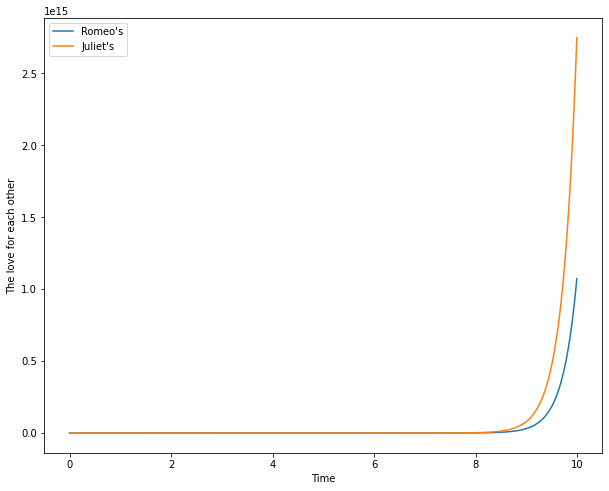
\includegraphics[scale = .33]{Images/Bt2/1.1_gr.png} & 
                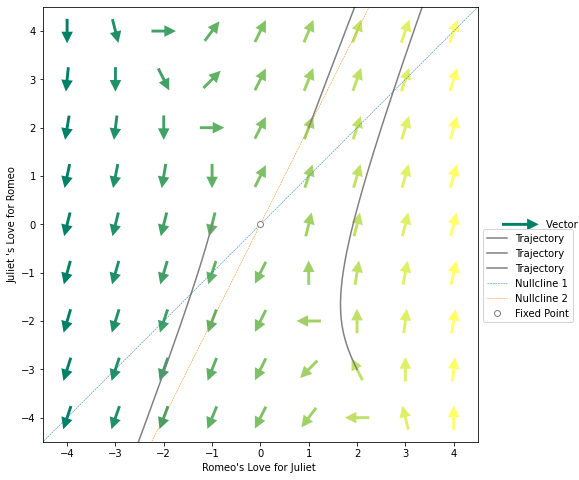
\includegraphics[scale = .33]{Images/Bt2/1.1_phase.png} \\ \\
                Đồ thị R, J theo t & Mặt phẳng pha 
            \end{tabular}
            \caption{The love between an eager beaver and an eager beaver}
        \end{figure}
        \item Với $a = 3,\;b = 4,\;c = 5,\;d = 4,\;R_0 = 1,\;J_0 = 5$ ta có hệ: 
        $$\begin{cases} \dot{R}=3R+4J \\ \dot{J}=5R+4J \\ R(0)=1,\;J(0)=5 \end{cases}$$ \\
        Áp dụng công thức (\ref{eq:11}) với $\Delta = 81 > 0$ ta có:
        $$\begin{cases}
            R = -\frac{5}{24}e^{-t} + \frac{1}{3} e^{8t} \\[4pt]
            J = \frac{5}{3}e^{-t} + \frac{10}{3}e^{8t}
        \end{cases}$$
        \begin{figure}[htp]
            \centering
            \begin{tabular}{cc}
                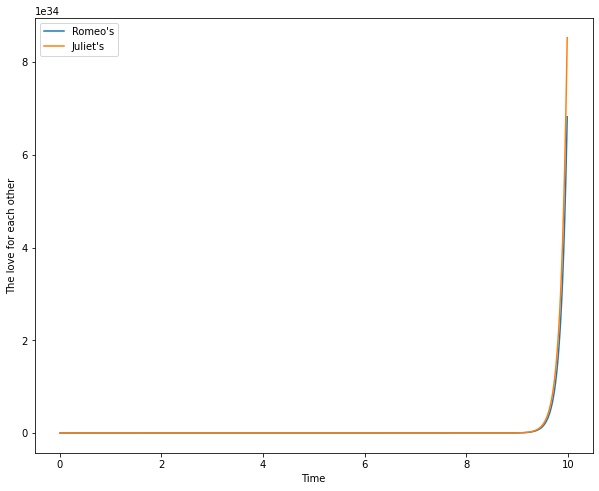
\includegraphics[scale = .33]{Images/Bt2/1.2_gr.png} &
                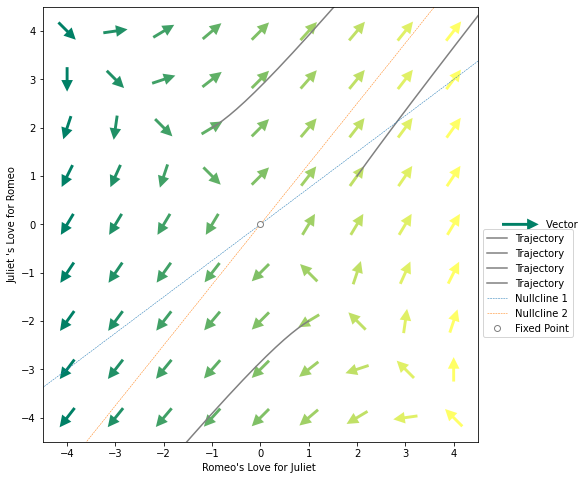
\includegraphics[scale = .33]{Images/Bt2/1.2_phase.png} \\
                Đồ thị R, J theo t & Mặt phẳng pha
            \end{tabular}
            \caption{The love between an eager beaver and an eager beaver}
        \end{figure}
    \end{itemize}
\item
Love between an eager beaver and a narcissistic nerd $(a,\;b,\;c > 0$ và $d < 0)$:
    \begin{itemize}
    \item Với $a = 2,\;b = 1,\;c = 1,\;d = -2,\;R_0 = 2,\;J_0 = 5$ ta có hệ:
    $$\begin{cases} \dot{R}=2R+J \\ \dot{J}=R-2J \\ R(0)=2,\;J(0)=0 \end{cases}$$ \\
    Áp dụng công thức (\ref{eq:11}) với $\Delta = 20 > 0$ ta có:
    $$\begin{cases}
        R = \frac{5+2\sqrt{5}}{5}e^{-\sqrt{5}t} + \frac{5-2\sqrt{5}}{5}e^{\sqrt{5}t} \\[4pt]
        J = -\frac{\sqrt{5}}{5}e^{-\sqrt{5}t} + \frac{\sqrt{5}}{5}e^{\sqrt{5}t}
    \end{cases}$$
    \begin{figure}[htp]
        \centering
        \begin{tabular}{cc}
            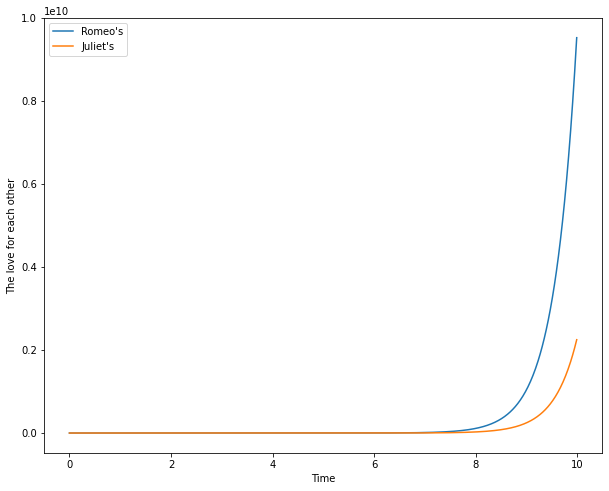
\includegraphics[scale = .33]{Images/Bt2/2.1_gr.png} &
            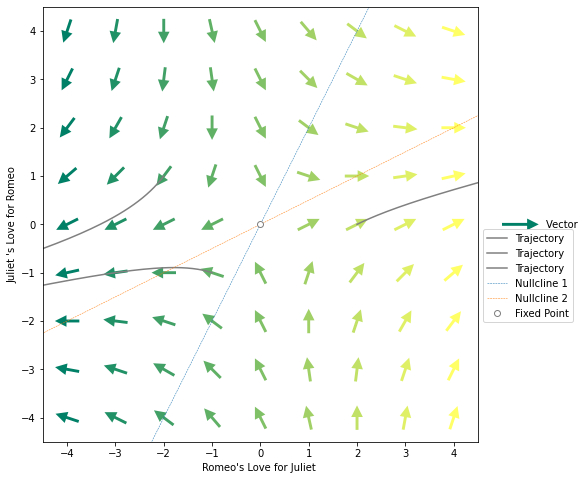
\includegraphics[scale = .33]{Images/Bt2/2.1_phase.png} \\
            Đồ thị R, J theo t & Mặt phẳng pha
        \end{tabular}
        \caption{The love between an eager beaver and a narcissistic nerd}
    \end{figure}
    \item Với $a = 1,\;b = 3,\;c = 2,\;d = -4,\;R_0 = 4,\;J_0 = -2$ ta có hệ:
    $$\begin{cases} \dot{R}=R+3J \\ \dot{J}=2R-4J \\ R(0)=4,\;J(0)=-2 \end{cases}$$ \\
    Áp dụng công thức (\ref{eq:11}) với $\Delta = 49 > 0$ ta có:
    $$\begin{cases}
        R = \frac{10}{7}e^{-5t} + \frac{18}{7}e^{2t} \\[3pt]
        J = -\frac{20}{7}e^{-5t} + \frac{6}{7}e^{2t}
    \end{cases}$$
    \begin{figure}[htp]
        \centering
        \begin{tabular}{cc}
            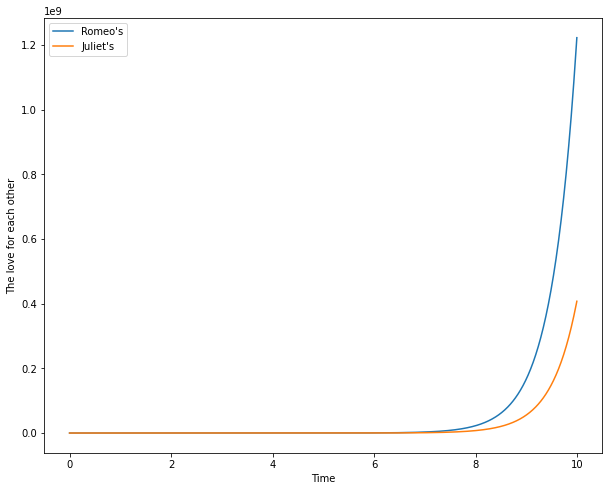
\includegraphics[scale = .33]{Images/Bt2/2.2_gr.png} &
            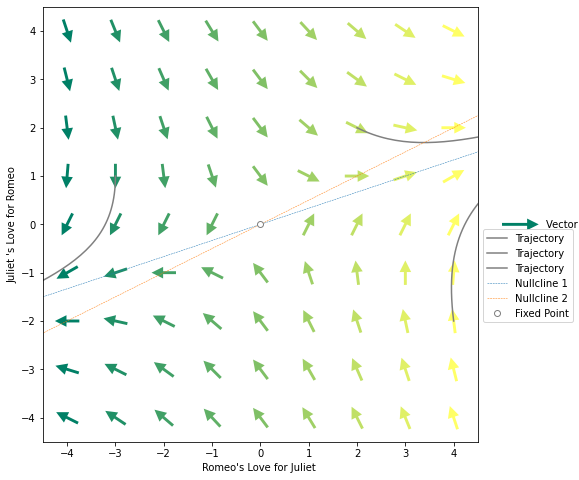
\includegraphics[scale = .33]{Images/Bt2/2.2_phase.png} \\
            Đồ thị R, J theo t & Mặt phẳng pha
        \end{tabular}
        \caption{The love between an eager beaver and a narcissistic nerd}
    \end{figure}
    \end{itemize}
\newpage
\item
Love between an eager beaver and a cautious lover $(a,\;b,\;c > 0$ và $d < 0)$ :
    \begin{itemize}
    \item Với $a = 3,\;b = 2,\;c = -2,\;d = 1,\;R_0 = 1,\;J_0 = 0$ ta có hệ:
    $$\begin{cases} \dot{R}=3R+2J \\ \dot{J}=-2R+J \\ R(0)=1,\;J(0)=0 \end{cases}$$ \\
    Áp dụng công thức (\ref{eq:24}) với $\Delta = -12 < 0$ ta có:
    $$\begin{cases}
        R = e^{2t}
        \left(\cos{t\sqrt{3}} + 
        \frac{\sqrt{3}}{3}\sin{t\sqrt{3}} \right) \\[4pt]
        J = -e^{2t} \frac{2\sqrt{3}}{3} \sin{t\sqrt{3}}
    \end{cases}$$
    \begin{figure}[htp]
        \centering
        \begin{tabular}{cc}
            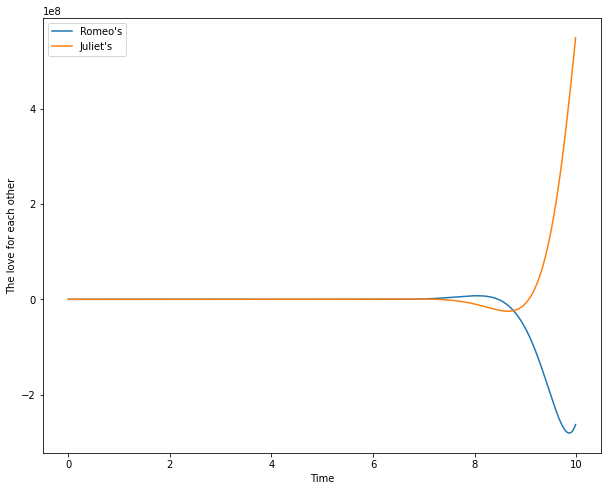
\includegraphics[scale = .33]{Images/Bt2/3.1_gr.png} &
            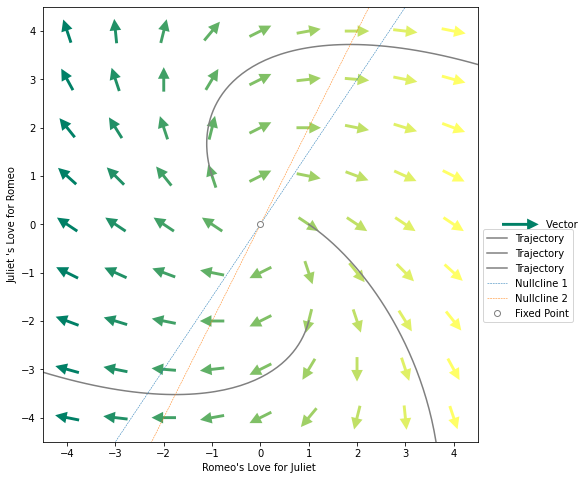
\includegraphics[scale = .33]{Images/Bt2/3.1_phase.png} \\
            Đồ thị R, J theo t & Mặt phẳng pha
        \end{tabular}
        \caption{The love between an eager beaver and a cautious lover}
    \end{figure}
    \item Với $a = 4,\;b = 1,\;c = -1,\;d = 2,\;R_0 = 4,\;J_0 = 3$ ta có hệ:
    $$\begin{cases} \dot{R}=4R+J \\ \dot{J}=-1R+2J \\ R(0)=4,\;J(0)=3 \end{cases}$$ \\
    Áp dụng công thức (\ref{eq:17}) với $\Delta = 0$ ta có:
    $$\begin{cases}
        R = (7t+4)e^{3t}\\
        J = (3-10t)e^{3t}
    \end{cases}$$
    \begin{figure}[htp]
        \centering
        \begin{tabular}{cc}
            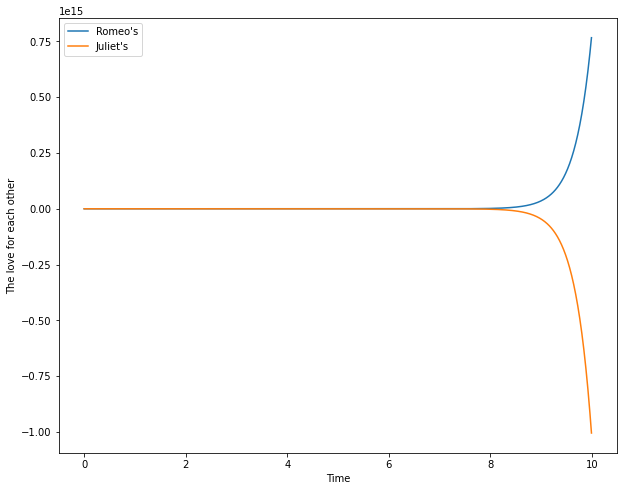
\includegraphics[scale = .33]{Images/Bt2/3.2_gr.png} &
            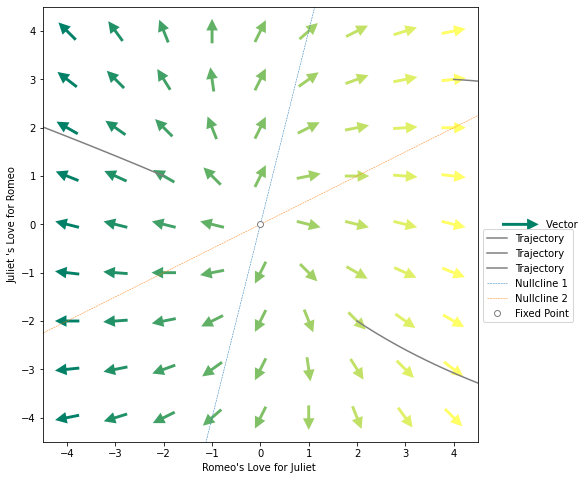
\includegraphics[scale = .33]{Images/Bt2/3.2_phase.png} \\
            Đồ thị R, J theo t & Mặt phẳng pha
        \end{tabular}
        \caption{The love between an eager beaver and a cautious lover}
    \end{figure}
    \end{itemize}
\newpage
\item
Love between an eager beaver and a hermit $(a,\;b > 0$ và $c,;d < 0)$:
    \begin{itemize}
    \item Với $a = 2,\;b = 4,\;c = -2,\;d = -2,\;R_0 = 0,\;J_0 = 3$ ta có hệ:
    $$\begin{cases} \dot{R}=2R+4J \\ \dot{J}=-2R-2J \\ R(0)=0,\;J(0)=3 \end{cases}$$ \\
    Áp dụng công thức (\ref{eq:24}) với $\Delta = -16 < 0$ ta có:
    $$\begin{cases}
        R = 6\sin{2t} \\
        J = 3\cos{2t} - 3\sin{2t}
    \end{cases}$$
    \begin{figure}[htp]
        \centering
        \begin{tabular}{cc}
            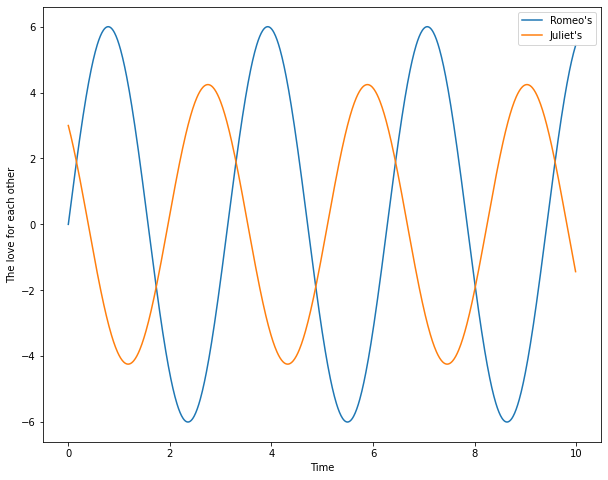
\includegraphics[scale = .33]{Images/Bt2/4.1_gr.png} &
            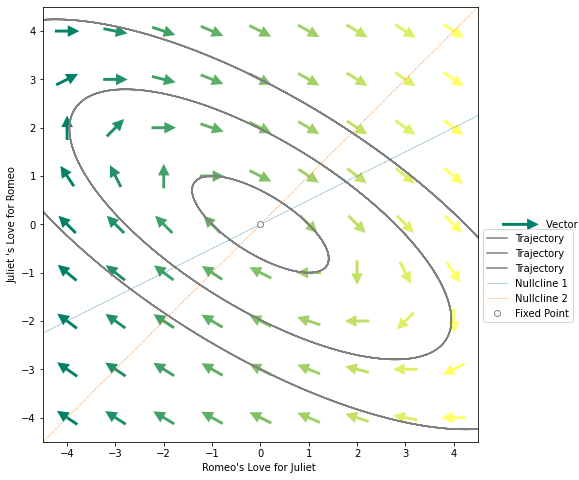
\includegraphics[scale = .33]{Images/Bt2/4.1_phase.png} \\
            Đồ thị R, J theo t & Mặt phẳng pha
        \end{tabular}
        \caption{The love between an eager beaver and a hermit}
    \end{figure}
    \item Với $a = 3,\;b = 3,\;c = -3,\;d = -3,\;R_0 = 1,\;J_0 = 0$ ta có hệ:
    $$\begin{cases} \dot{R}=3R+3J \\ \dot{J}=-3R-3J \\ R(0)=1,\;J(0)=0 \end{cases}$$ \\
    Áp dụng công thức (\ref{eq:17}) với $\Delta = 0$ ta có:
    $$\begin{cases}
        R = 3t + 1 \\
        J = -3t
    \end{cases}$$
    Đây là một trường hợp đặc biệt khi cả $\Delta$ và $\lambda$ đều bằng $0$, hàm số $R(t)$, $J(t)$ suy biến từ hàm mũ thành hàm tuyến tính.
    \begin{figure}[htp]
        \centering
        \begin{tabular}{cc}
            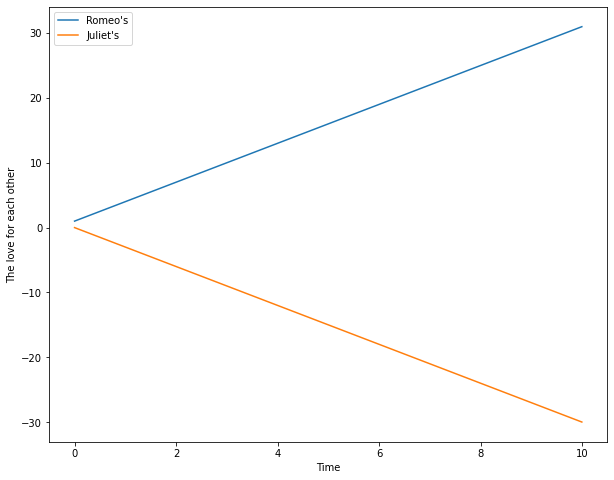
\includegraphics[scale = .33]{Images/Bt2/4.2_gr.png} &
            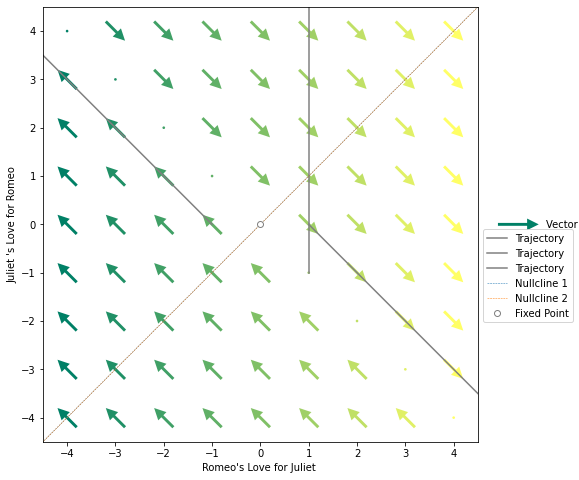
\includegraphics[scale = .33]{Images/Bt2/4.2_phase.png} \\
            Đồ thị R, J theo t & Mặt phẳng pha
        \end{tabular}
        \caption{The love between an eager beaver and a hermit}
    \end{figure}
    \end{itemize}
\newpage
\item
Love between a narcissistic nerd and a narcissistic nerd $(a,\;c > 0$ và $b,\;d < 0)$ :
    \begin{itemize}
    \item Với $a = 2,\;b = -3,\;c = 3,\;d = -4,\;R_0 = 2,\;J_0 = -2$ ta có hệ:
    $$\begin{cases} \dot{R}=2R-3J \\ \dot{J}=3R-4J \\ R(0)=2,\;J(0)=-2 \end{cases}$$ \\
    Áp dụng công thức (\ref{eq:17}) với $\Delta = 0$ ta có:
    $$\begin{cases}
        R = \left( 2 - 12t \right)e^{-t} \\
        J = -\left( 18t + 2 \right)e^{-t} \\
    \end{cases}$$
    \begin{figure}[htp]
        \centering
        \begin{tabular}{cc}
            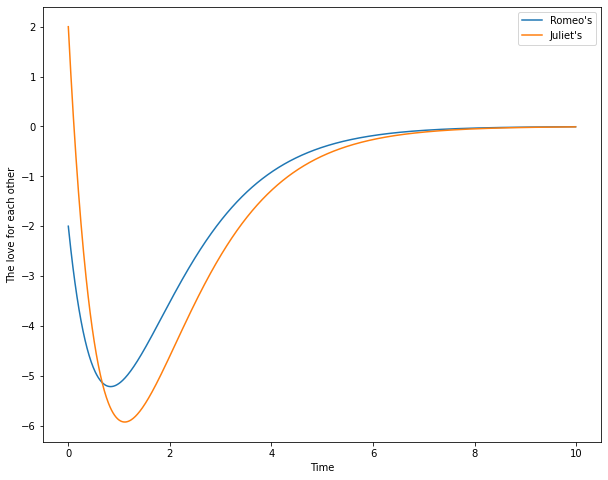
\includegraphics[scale = .33]{Images/Bt2/5.1_gr.png} &
            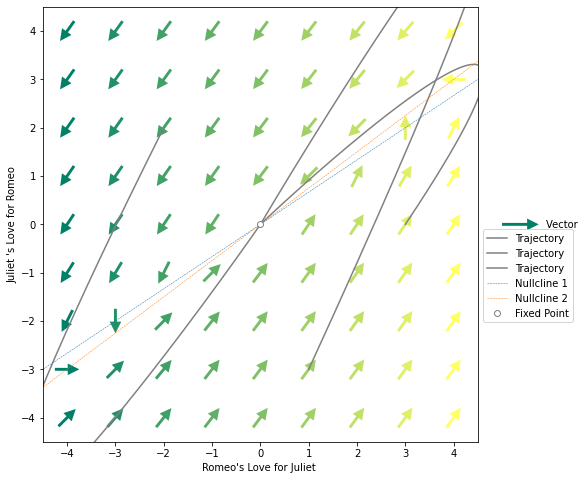
\includegraphics[scale = .33]{Images/Bt2/5.1_phase.png} \\
            Đồ thị R, J theo t & Mặt phẳng pha
        \end{tabular}
        \caption{The love between a narcissistic nerd and a narcissistic nerd}
    \end{figure}
    \item Với $a = 1,\;b = -2,\;c = 4,\;d = -3,\;R_0 = 2,\;J_0 = 3$ ta có hệ:
    $$\begin{cases} \dot{R}=R-2J \\ \dot{J}=4R-3J \\ R(0)=2,\;J(0)=3 \end{cases}$$ \\
    Áp dụng công thức (\ref{eq:24}) với $\Delta = -16 < 0$ ta có:
    $$\begin{cases}
        R = e^{-t}\left(2 \cos{2t} - \sin{2t} \right) \\
        J = e^{-t}\left(3 \cos{2t} + \sin{2t} \right) \\
    \end{cases}$$
    \begin{figure}[htp]
        \centering
        \begin{tabular}{cc}
            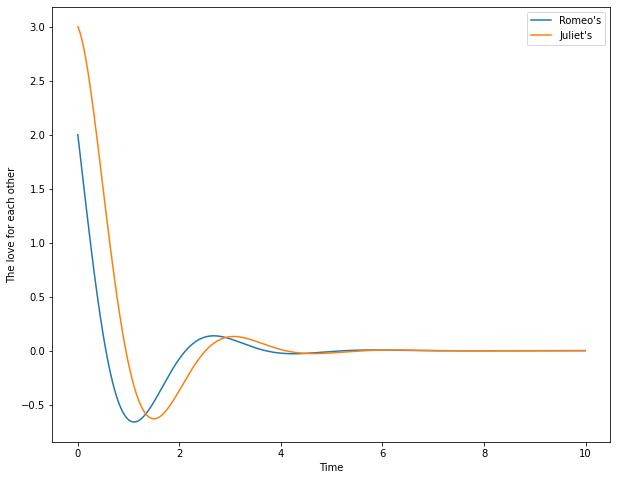
\includegraphics[scale = .33]{Images/Bt2/5.2_gr.png} &
            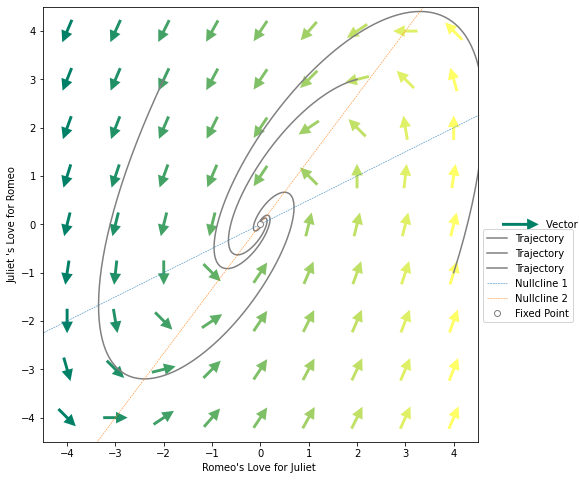
\includegraphics[scale = .33]{Images/Bt2/5.2_phase.png} \\
            Đồ thị R, J theo t & Mặt phẳng pha
        \end{tabular}
        \caption{The love between a narcissistic nerd and a narcissistic nerd}
    \end{figure}
    \end{itemize}
\item
Love between a narcissistic nerd and a cautious lover $(a,\;d > 0$ và $b,\;c < 0)$ :
    \begin{itemize}
    \item Với $a = 1,\;b = -2,\;c = -1,\;d = 2,\;R_0 = 0,\;J_0 = 3$ ta có hệ:
    $$\begin{cases} \dot{R}=R-2J \\ \dot{J}=-R+2J \\ R(0)=0,\;J(0)=3 \end{cases}$$ \\
    Áp dụng công thức (\ref{eq:11}) với $\Delta = 9 > 0$ ta có:
    $$\begin{cases}
        R = 2 + 2e^{3t} \\
        J = 1 + 2e^{3t}
    \end{cases}$$
    \begin{figure}[htp]
        \centering
        \begin{tabular}{cc}
            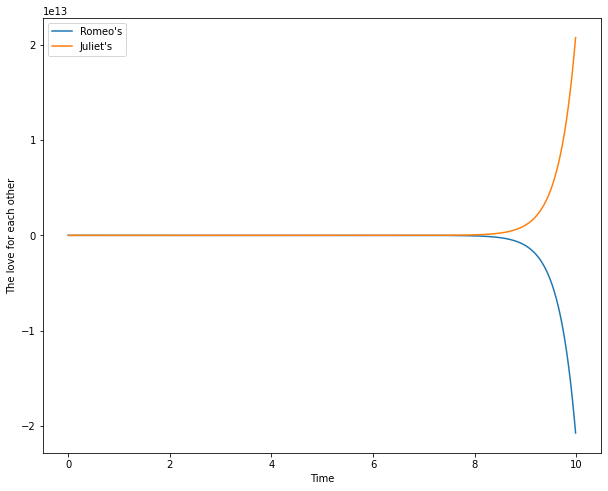
\includegraphics[scale = .33]{Images/Bt2/6.1_gr.png} &
            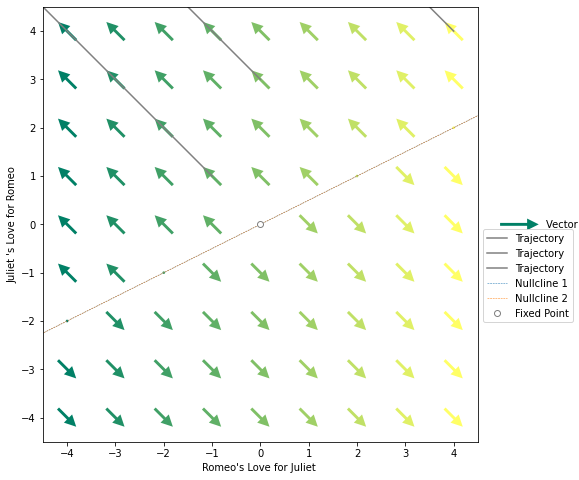
\includegraphics[scale = .33]{Images/Bt2/6.1_phase.png} \\
            Đồ thị R, J theo t & Mặt phẳng pha
        \end{tabular}
        \caption{The love between a narcissistic nerd and a cautious lover}
    \end{figure}
\newpage
    \item Với $a = 2,\;b = -3,\;c = -2,\;d = 1,\;R_0 = 0,\;J_0 = 4$ ta có hệ:
    $$\begin{cases} \dot{R}=2R-3J \\ \dot{J}=-2R+J \\ R(0)=0,\;J(0)=4 \end{cases}$$ \\
    Áp dụng công thức (\ref{eq:11}) với $\Delta = 25 > 0$ ta có:
    $$\begin{cases}
        R = \frac{12}{5}e^{-t} - \frac{12}{5}e^{4t} \\[3pt]
        J = \frac{12}{5}e^{-t} + \frac{8}{5}e^{4t}
    \end{cases}$$
    \begin{figure}[htp]
        \centering
        \begin{tabular}{cc}
            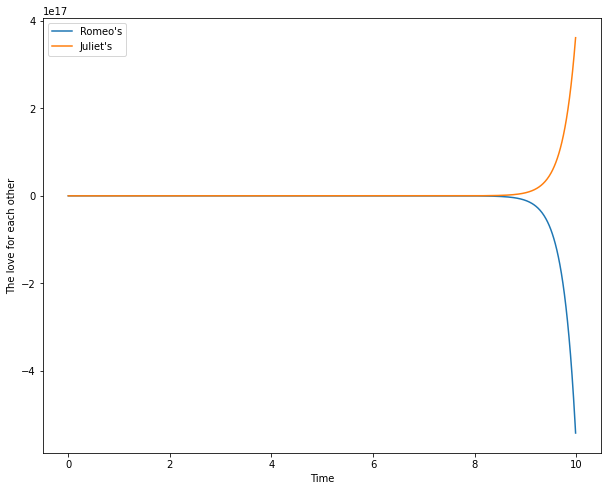
\includegraphics[scale = .33]{Images/Bt2/6.2_gr.png} &
            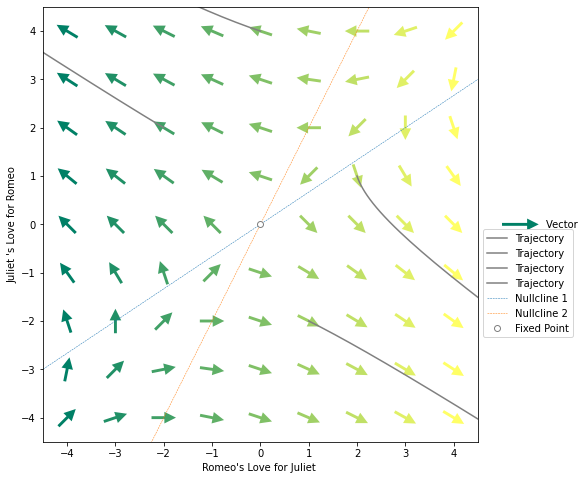
\includegraphics[scale = .33]{Images/Bt2/6.2_phase.png} \\
            Đồ thị R, J theo t & Mặt phẳng pha
        \end{tabular}
        \caption{The love between a narcissistic nerd and a cautious lover}
    \end{figure}
    \end{itemize}
\item
Love between a narcissistic nerd and a hermit $(a > 0$ và $b,\;c,\;d < 0)$ :
    \begin{itemize}
    \item Với $a = 2,\;b = -2,\;c = -2,\;d = -1,\;R_0 = 2,\;J_0 = 4$ ta có hệ:
    $$\begin{cases} \dot{R}=2R-2J \\ \dot{J}=-2R-J \\ R(0)=2,\;J(0)=4 \end{cases}$$ \\
    Áp dụng công thức (\ref{eq:11}) với $\Delta = 25 > 0$ ta có:
    $$\begin{cases}
        R = 2e^{-2t} \\
        J = 4e^{-2t}
    \end{cases}$$
    \begin{figure}[htp]
        \centering
        \begin{tabular}{cc}
            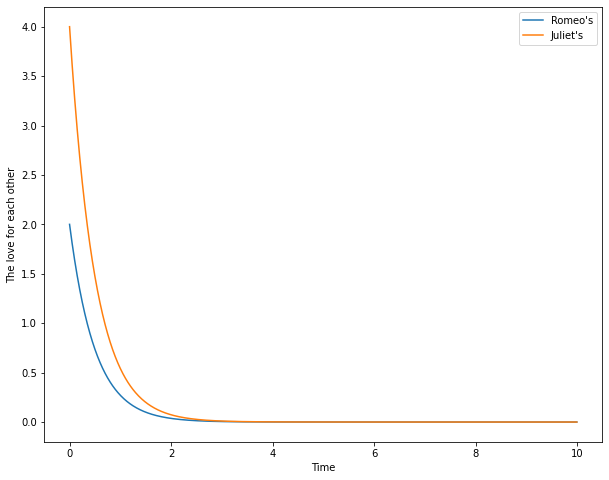
\includegraphics[scale = .33]{Images/Bt2/7.1_gr.png} &
            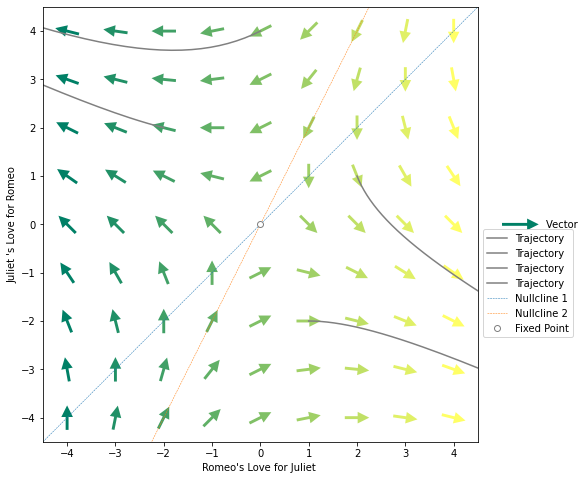
\includegraphics[scale = .33]{Images/Bt2/7.1_phase.png} \\
            Đồ thị R, J theo t & Mặt phẳng pha
        \end{tabular}
        \caption{The love between a narcissistic nerd and a hermit}
    \end{figure}
    \item Với $a = 2,\;b = -1,\;c = -3,\;d = -2,\;R_0 = 2,\;J_0 = 4$ ta có hệ:
    $$\begin{cases} \dot{R}=2R-J \\ \dot{J}=-3R-2J \\ R(0)=2,\;J(0)=4 \end{cases}$$ \\
    Áp dụng công thức (\ref{eq:11}) với $\Delta = 28 > 0$ ta có:
    $$\begin{cases}
        R = e^{-t\sqrt{7}} - e^{t\sqrt{7}} \\
        J = -(2+\sqrt{7})e^{-t\sqrt{7}} - (2-\sqrt{7})e^{t\sqrt{7}}
    \end{cases}$$
    \begin{figure}[htp]
        \centering
        \begin{tabular}{cc}
            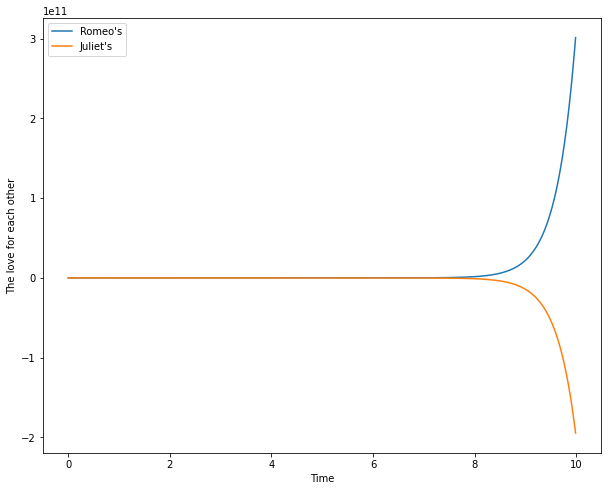
\includegraphics[scale = .33]{Images/Bt2/7.2_gr.png} &
            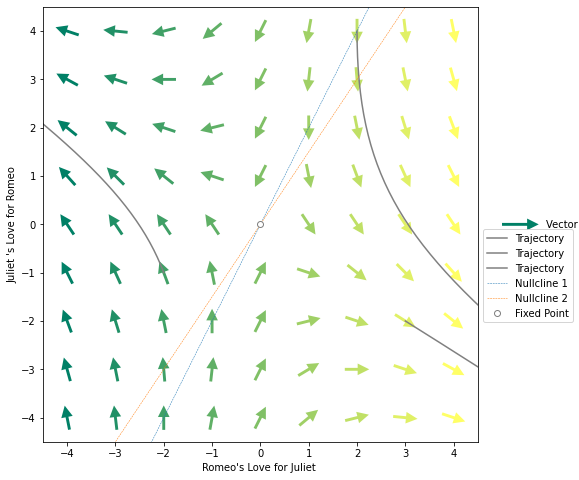
\includegraphics[scale = .33]{Images/Bt2/7.2_phase.png} \\
            Đồ thị R, J theo t & Mặt phẳng pha
        \end{tabular}
        \caption{The love between a narcissistic nerd and a hermit}
    \end{figure}
    \end{itemize}
\newpage
\item
Love between a cautious lover and a cautious lover $(b,\;d > 0$ và $a,\;c < 0)$:
    \begin{itemize}
    \item Với $a = -3,\;b = 3,\;c = -2,\;d = 1,\;R_0 = -4,\;J_0 = 2$ ta có hệ:
    $$\begin{cases} \dot{R}=-3R+3J \\ \dot{J}=-2R+J \\ R(0)=-4,\;J(0)=2 \end{cases}$$ \\
    Áp dụng công thức (\ref{eq:24}) với $\Delta = -8 < 0$ ta có:
    $$\begin{cases}
        R = e^{-t}\left[ 7\sqrt{2}\sin{\left( t\sqrt{2} \right)} - 4\cos{\left( t\sqrt{2} \right)}\right] \\[3pt]
        J = e^{-t}\left[ 2\cos{\left( t\sqrt{2} \right)} + 6\sqrt{2}\sin{\left( t\sqrt{2} \right)}\right]
    \end{cases}$$
    \begin{figure}[htp]
        \centering
        \begin{tabular}{cc}
            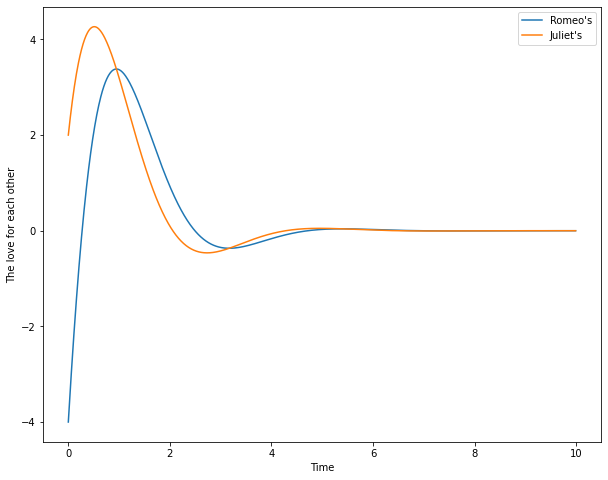
\includegraphics[scale = .33]{Images/Bt2/8.1_gr.png} &
            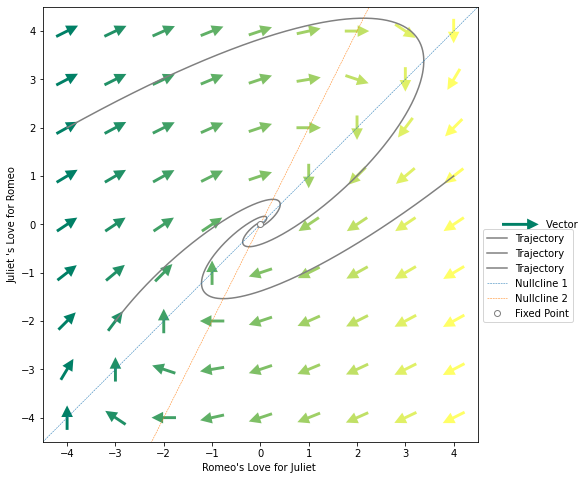
\includegraphics[scale = .33]{Images/Bt2/8.1_phase.png} \\
            Đồ thị R, J theo t & Mặt phẳng pha
        \end{tabular}
        \caption{The love between a cautious lover and a cautious lover}
    \end{figure}
    \item Với $a = -4,\;b = 3,\;c = -3,\;d = 2,\;R_0 = 4,\;J_0 = 0$ ta có hệ:
    $$\begin{cases} \dot{R}=-4R+3J \\ \dot{J}=-3R+2J \\ R(0)=4,\;J(0)=0 \end{cases}$$ \\
    Áp dụng công thức (\ref{eq:17}) với $\Delta = 0$ ta có:
    $$\begin{cases}
        R = (4 - 12t)e^{-t} \\
        J = -12e^{-t} \\
    \end{cases}$$
    \begin{figure}[htp]
        \centering
        \begin{tabular}{cc}
            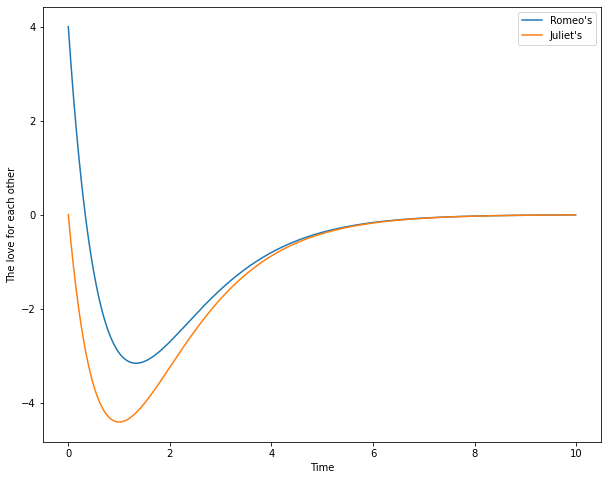
\includegraphics[scale = .33]{Images/Bt2/8.2_gr.png} &
            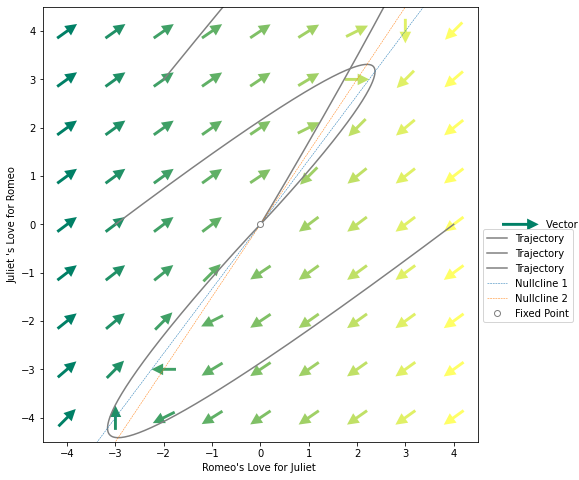
\includegraphics[scale = .33]{Images/Bt2/8.2_phase.png} \\
            Đồ thị R, J theo t & Mặt phẳng pha
        \end{tabular}
        \caption{The love between a cautious lover and a cautious lover}
    \end{figure}
    \end{itemize}
\newpage
\item
Love between a cautious lover and a hermit $(b > 0$ và $a,\;c,\;d < 0)$:
    \begin{itemize}
    \item Với $a = -2,\;b = 4,\;c = -4,\;d = -2,\;R_0 = -2,\;J_0 = 2$ ta có hệ:
    $$\begin{cases} \dot{R}=-2R+4J \\ \dot{J}=-4R-2J \\ R(0)=-2,\;J(0)=2 \end{cases}$$ \\
    Áp dụng công thức (\ref{eq:24}) với $\Delta = -64 < 0$ ta có:
    $$\begin{cases}
        R = e^{-t}\left[ 4\sin{\left( 4t \right)} - 2\cos{\left( 4t \right)}\right] \\
        J = e^{-t}\left[ 2\cos{\left( 4t \right)} - 2\sin{\left( 4t \right)}\right]
    \end{cases}$$
    \begin{figure}[htp]
        \centering
        \begin{tabular}{cc}
            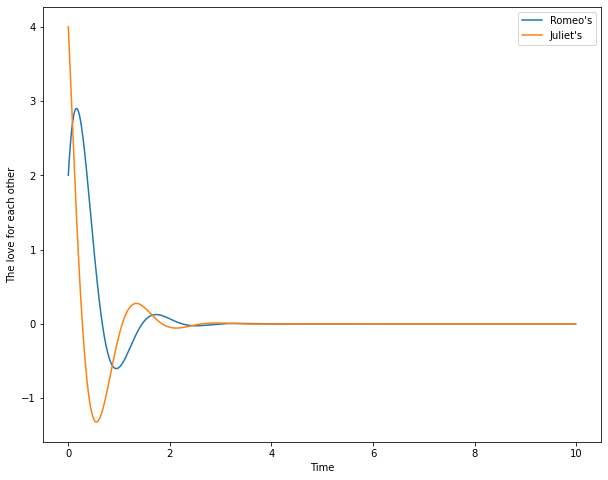
\includegraphics[scale = .33]{Images/Bt2/9.1_gr.png} &
            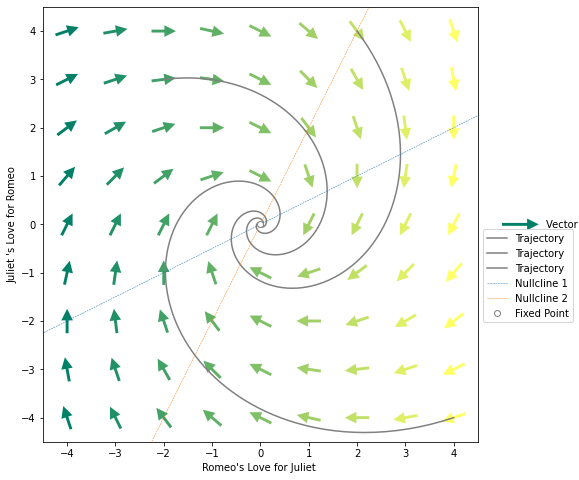
\includegraphics[scale = .33]{Images/Bt2/9.1_phase.png} \\
            Đồ thị R, J theo t & Mặt phẳng pha
        \end{tabular}
        \caption{The love between a cautious lover and a hermit}
    \end{figure}
    \item Với $a = -4,\;b = 1,\;c = -2,\;d = -1,\;R_0 = -4,\;J_0 = 4$ ta có hệ:
    $$\begin{cases} \dot{R}=-4R+J \\ \dot{J}=-2R-J \\ R(0)=-4,\;J(0)=4 \end{cases}$$ \\
    Áp dụng công thức (\ref{eq:11}) với $\Delta = 1 > 0$ ta có:
    $$\begin{cases}
        R = -12e^{-3t} + 8e^{-2t} \\
        J = -18e^{-3t} + 16e^{-2t}
    \end{cases}$$
    \begin{figure}[htp]
        \centering
        \begin{tabular}{cc}
            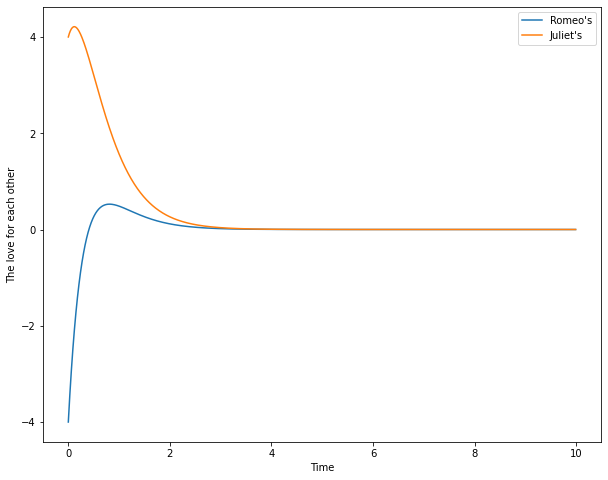
\includegraphics[scale = .33]{Images/Bt2/9.2_gr.png} &
            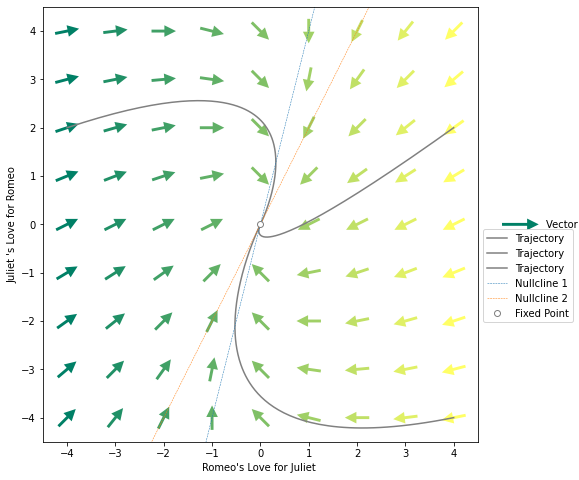
\includegraphics[scale = .33]{Images/Bt2/9.2_phase.png} \\
            Đồ thị R, J theo t & Mặt phẳng pha
        \end{tabular}
        \caption{The love between a cautious lover and a hermit}
    \end{figure}
    \end{itemize}
\newpage
\item
Love between a hermit and a hermit $(a,\;b,\;c,\;d < 0)$:
    \begin{itemize}
    \item Với $a = -4,\;b = -1,\;c = -2,\;d = -2,\;R_0 = 0,\;J_0 = 4$ ta có hệ:
    $$\begin{cases} \dot{R}=-4R-J \\ \dot{J}=-2R-2J \\ R(0)=0,\;J(0)=4 \end{cases}$$ \\
    Áp dụng công thức (\ref{eq:11}) với $\Delta = 12 > 0$ ta có:
    $$\begin{cases}
        R = \frac{2\sqrt{3}}{3}e^{-(3+\sqrt{3})t} - \frac{2\sqrt{3}}{3}e^{(\sqrt{3}-3)t} \\[4pt]
        J = \frac{6-2\sqrt{3}}{3}e^{-(3+\sqrt{3})t} - \frac{6+2\sqrt{3}}{3}e^{(\sqrt{3}-3)t}
    \end{cases}$$
    \begin{figure}[htp]
        \centering
        \begin{tabular}{cc}
            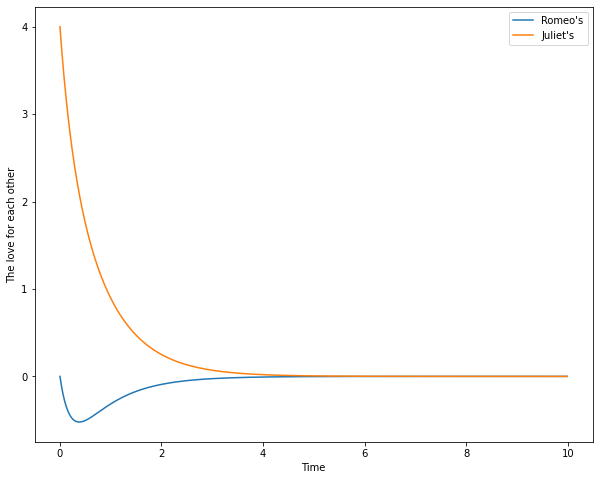
\includegraphics[scale = .33]{Images/Bt2/10.1_gr.png} &
            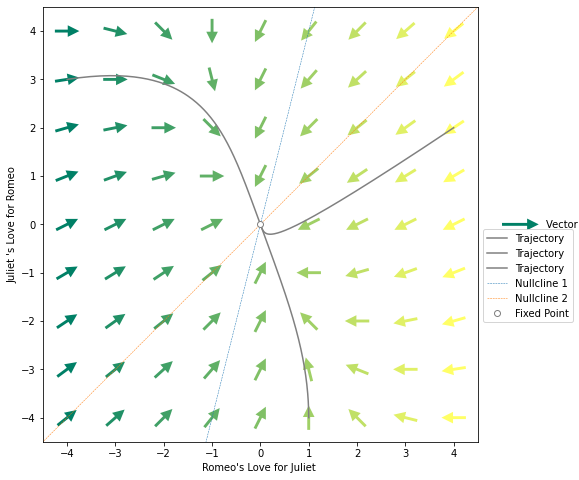
\includegraphics[scale = .33]{Images/Bt2/10.1_phase.png} \\
            Đồ thị R, J theo t & Mặt phẳng pha
        \end{tabular}
        \caption{The love between a hermit and a hermit}
    \end{figure}
    \item Với $a = -2,\;b = -3,\;c = -4,\;d = -2,\;R_0 = 0,\;J_0 = 4$ ta có hệ:
    $$\begin{cases} \dot{R}=-2R-3J \\ \dot{J}=-4R-2J \\ R(0)=0,\;J(0)=4 \end{cases}$$ \\
    Áp dụng công thức (\ref{eq:11}) với $\Delta = 48 > 0$ ta có:
    \begin{equation*}
        \begin{cases}
        R = \sqrt{3}e^{-(2+2\sqrt{3})t} - \sqrt{3}e^{(2\sqrt{3}-2)t} \\[4pt]
        J = 2e^{-(2+2\sqrt{3})t} + 2e^{(2\sqrt{3}-2)t}
    \end{cases}
    \end{equation*}
    \begin{figure}[htp]
        \centering
        \begin{tabular}{cc}
            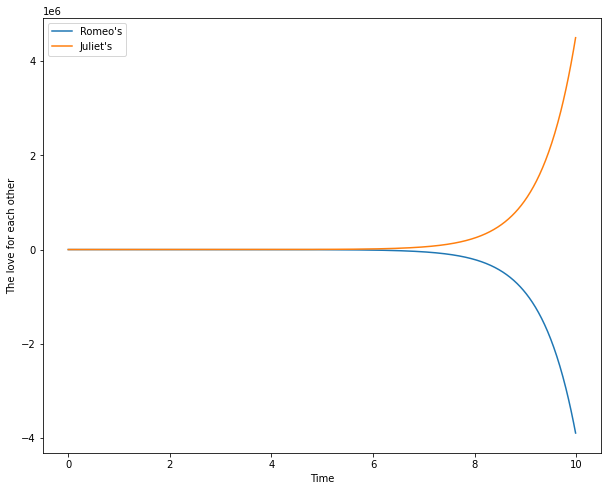
\includegraphics[scale = .33]{Images/Bt2/10.2_gr.png} &
            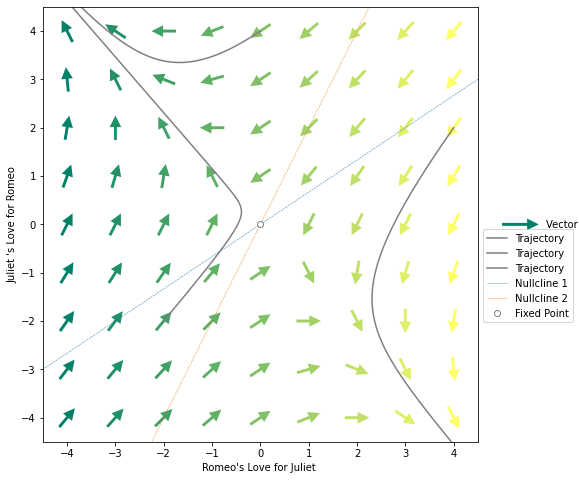
\includegraphics[scale = .33]{Images/Bt2/10.2_phase.png} \\
            Đồ thị R, J theo t & Mặt phẳng pha
        \end{tabular}
        \caption{The love between a hermit and a hermit}
    \end{figure}
    \end{itemize}
\end{enumerate}
\newpage
\subsection{Bài tập 3:} \label{ex:3}
\subsubsection{Nonhomogeneous Linear Systems of Differential Equations}
\subsubsubsection{Nghiệm của hệ}
$\indent$ Coi như tình yêu giữa Romeo và Juliet giờ đây không còn là nghiệm của hệ phương trình vi phân tuyến tính như ở hệ (\ref{eq:1}) mà có nhân tố ngoài ảnh hưởng và được biểu diễn bởi hệ phương trình vi phân cấp một không thuần nhất như hệ sau:
\begin{equation} \label{eq:25}
    \left\{\begin{array}{@{}l@{}}
        \dot{R} = aR + bJ + f (t) \\
        \dot{J} =  cR + dJ + g(t) \\
        R(0) = R_{0}, J(0) = J_{0}.
    \end{array}\right.\,.
\end{equation}
Hay:
\begin{equation*}
    \left\{\begin{array}{@{}l@{}}
        \left( \begin{matrix} \dot {R} \\ \dot{J} \end{matrix} \right) = 
        \left( \begin{matrix} a & b \\ c & d \end{matrix} \right)
        \left( \begin{matrix} R \\ J \end{matrix} \right) + \left( \begin{matrix} f(t) \\ g(t) \end{matrix} \right) \\[10pt]
        R(0) = R_{0}, J(0) = J_{0}.
    \end{array}\right.\,.
\end{equation*}
\begin{itemize}
\item Đặt: $x(t) = \left( \begin{matrix} R \\ J \end{matrix} \right)$, $  A =  \left( \begin{matrix} a & b \\ c & d  \end{matrix} \right) $ và $ b(t) = \left( \begin{matrix} f(t) \\ g(t) \end{matrix} \right)$ :
    \begin{equation} \label{eq:26} 
        \dot{x}(t) = Ax(t) + b(t)
    \end{equation}
\item Để tìm được nghiệm cho hệ phương trình tuyến tính không thuận nhất, ta làm theo các bước sau:
    \begin{enumerate} [(1)]
    \item
        Tìm nghiệm tổng quát $x_c(t) = \phi(t)c$ cho hệ phương trình vi phân tuyến tính thuần nhất $x'(t) = Ax(t)$, trong đó $\phi(t)$ là ma trận cơ bản.
    \item
        Tìm 1 nghiệm riêng 
        \begin{equation} \label{eq:27}
        x_p(t) = \phi(t)\int\phi(t)^{-1}b(t)dt
        \end{equation}
        \item Nghiệm tổng quát của hệ phương trình vi phân tuyến tính không thuần nhất là:
        \begin{equation} \label{eq:28}
        x(t) = x_c(t) + x_p(t)
        \end{equation}
    \end{enumerate}
    
\item Chứng minh (\ref{eq:27}):
    \begin{itemize} 
    \item[-] Ta tìm nghiệm riêng $x_p(t) = \phi(t)u$, trong đó $\phi(t)$ là ma trận cơ bản và u là vector hàm cần được tìm, thế vào (\ref{eq:26}):
        \begin{equation*}
            \begin{split}
                &(\phi(t)u)' = A\phi(t)u + b(t)\\
                \implies &\phi'(t)u + \phi(t)\dot{u} = A\phi(t)u + b(t)\\
                \implies &A\phi(t)u + \phi(t)\dot{u} = A\phi(t)u + b(t)\\
                \implies &\phi(t)\dot{u} = b(t)\\
                \implies &\dot{u} = \phi(t)^{-1}b(t) \\
                \implies &u = \int\phi(t)^{-1}b(t)dt
            \end{split}
        \end{equation*}
    \item[-] Vậy, ta được: $x_p(t) = \phi(t)\int\phi(t)^{-1}b(t)dt$
    \end{itemize}
\item Chứng minh (\ref{eq:28}):
    \begin{equation*}
        \begin{split}
            &(x_c(t) + x_p(t))' = x_c'(t) + x_p'(t)\\
            \implies &(x_c(t) + x_p(t))' = Ax_c(t) + Ax_p(t) + b(t)\\
            \implies &(x_c(t) + x_p(t))' = A(x_c(t) + x_p(t)) + b(t)
        \end{split}
    \end{equation*}
    \begin{itemize}
    \item Vậy (\ref{eq:28}) là nghiệm của (\ref{eq:26}).
    \end{itemize}
\item Vậy để hệ phương trình vi phân tuyến tính không thuần nhất có nghiệm tổng quát thì: b(t) phải là vector gồm những hàm liên tục trên khoảng xác định và có nguyên hàm cơ bản. \\
\textbf{Lưu ý:} Một số hàm dù không có nguyên hàm cơ bản nhưng ta vẫn có thể dùng công thức trên để tính ra đáp án.
\end{itemize}
\subsubsubsection{Ví dụ}
\begin{enumerate}
\item Ví dụ 1:   $$\left\{\begin{array}{@{}l@{}}
            \dot{R} = R + 2J - t \\
            \dot{J} =  3R + 2J + 3t^2 \\
            R(0) = 0, J(0) = 4
        \end{array}\right.$$
    \begin{itemize}
    \item Áp dụng kết quả từ câu 1, ta tìm được nghiệm tổng quát $x_c(t)$ của hệ phương trình vi phân tuyến tính thuần nhất có được từ hệ phương trình để bài và có được ma trận cơ bản là:
        \begin{center}
            $x_c(t) = \left( \begin{matrix} 2e^{4t} & -e^{-t} \\ 3e^{4t} & e^{-t} \end{matrix} \right) \left( \begin{matrix} C_1 \\ C_2 \end{matrix} \right)$ và $\phi(t) = \left( \begin{matrix} 2e^{4t} & -e^{-t} \\ 3e^{4t} & e^{-t} \end{matrix} \right)$
        \end{center}
    \item Sau đó ta đi tính \\ $\phi^{-1}(t) = \left( \begin{matrix} \frac{e^{-4t}}{5} & \frac{e^{-4t}}{5} \\[2pt] -\frac{3e^{t}}{5} & \frac{2e^{t}}{5} \end{matrix} \right)$ và $\int\phi^{-1}(t)b(t)dt = \left( \begin{matrix} -\frac{(1+4t+24t^2)e^{-4t}}{160} \\[2pt] \frac{3(2t^2-3t+3)e^t}{5} \end{matrix} \right)$
    \item Ta được nghiệm riêng $ x_p(t) = \phi(t)\int\phi(t)^{-1}b(t)dt = \left( \begin{matrix} -\frac{24t^2-28t+29}{16} \\[2pt] \frac{24t^2-60t+57}{32} \end{matrix} \right)$
    \item Suy ra nghiệm tổng quát của hệ phương trình đề bài là:
        \begin{center}
                $ x(t) = x_c(t) + x_p(t) = \left( \begin{matrix} 2e^{4t} & -e^{-t} \\ 3e^{4t} & e^{-t} \end{matrix} \right) \left( \begin{matrix} C_1 \\ C_2 \end{matrix} \right) + \left( \begin{matrix} -\frac{24t^2-28t+29}{16} \\[2pt] \frac{24t^2-60t+57}{32} \end{matrix} \right)$,
        \end{center}
        thế t = 0, R(0) = 0, J(0) = 4 vào, ta tính được $\left( \begin{matrix} C_1 \\ C_2 \end{matrix} \right) = \left( \begin{matrix} -\frac{127}{160} \\[2pt] -\frac{17}{5} \end{matrix} \right)$ 
    \item Vậy nghiệm tổng quát của hệ phương trình đề bài là: 
        \begin{center}
                $ x(t) = x_c(t) + x_p(t) = \left( \begin{matrix} 2e^{4t} & -e^{-t} \\ 3e^{4t} & e^{-t} \end{matrix} \right) \left( \begin{matrix} -\frac{127}{160} \\[2pt] -\frac{17}{5} \end{matrix} \right) + \left( \begin{matrix} -\frac{24t^2-28t+29}{16} \\[2pt] \frac{24t^2-60t+57}{32} \end{matrix} \right)$,
        \end{center}
    \end{itemize}
\item Ví dụ 2  $$\left\{\begin{array}{@{}l@{}}
            \dot{R} = 3R - 4J + e^t \\
            \dot{J} =  R + J + e^t \\
            R(0) = 1, J(0) = 1
        \end{array}\right.$$
    \begin{itemize}
    \item Áp dụng kết quả từ câu 1, ta tìm được nghiệm tổng quát $x_c(t)$ của hệ phương trình vi phân tuyến tính thuần nhất có được từ hệ phương trình để bài và có được ma trận cơ bản là:
        \begin{center}
            $x_c(t) = \left( \begin{matrix} 2e^{t} & (1+2t)e^{t} \\ e^{t} & te^{t} \end{matrix} \right) \left( \begin{matrix} C_1 \\ C_2 \end{matrix} \right)$ và $\phi(t) = \left( \begin{matrix} 2e^{t} & (1+2t)e^{t} \\ e^{t} & te^{t} \end{matrix} \right)$
        \end{center}
    \item Sau đó ta đi tính
        \begin{center}
            $\phi^{-1}(t) = \left( \begin{matrix} -te^{-t} & (1+2t)e^{-t} \\ e^{-t} & -2e^{-t} \end{matrix} \right)$ và $\int\phi^{-1}(t)b(t)dt = \left( \begin{matrix} \frac{t^2}{2} + t \\ -t \end{matrix} \right)$
        \end{center}
    \item Ta được nghiệm riêng $$x_p(t) = \phi(t)\int\phi(t)^{-1}b(t)dt = e^{t}t \left( \begin{matrix} 1-t \\ 4-2t \end{matrix} \right)$$
    \item Suy ra nghiệm tổng quát của hệ phương trình đề bài là:
        \begin{center}
                $x(t) = x_c(t) + x_p(t) = \left( \begin{matrix} 2e^{t} & (1+2t)e^{t} \\ e^{t} & te^{t} \end{matrix} \right) \left( \begin{matrix} C_1 \\ C_2 \end{matrix} \right) + e^{t}t \left( \begin{matrix} 1-t\\ 4-2t \end{matrix} \right)$
        \end{center}
        Thế t = 0, R(0) = 1, J(0) = 1 vào, ta tính được $\left( \begin{matrix} C_1 \\ C_2 \end{matrix} \right) = \left( \begin{matrix} 1 \\ 0 \end{matrix} \right)$ 
    \item Vậy nghiệm tổng quát của hệ phương trình đề bài là: 
        \begin{center}
                $x(t) = x_c(t) + x_p(t) = \left( \begin{matrix} 2e^{t} & (1+2t)e^{t} \\ e^{t} & te^{t} \end{matrix} \right) \left( \begin{matrix}{c} 1 \\ 0 \end{matrix} \right) + e^{t}t \left( \begin{matrix} 1-t\\ 4-2t \end{matrix} \right)$,
        \end{center}
    \end{itemize}
\item Ví dụ 3  $$\left\{\begin{array}{@{}l@{}}
            \dot{R} = 3R + 9J + \sin{t} \\
            \dot{J} =  -4R - 3J + \cos{t} \\
            R(0) = 2, J(0) = -4
        \end{array}\right.$$
    \begin{itemize}
    \item Áp dụng kết quả từ câu 1, ta tìm được nghiệm tổng quát $x_c(t)$ của hệ phương trình vi phân tuyến tính thuần nhất có được từ hệ phương trình để bài và có được ma trận cơ bản là:
        $$x_c(t) = \left( \begin{matrix} 3\cos{3\sqrt{3}t} & 3\sin{3\sqrt{3}t} \\ -\cos{3\sqrt{3}t} - \sqrt{3}\sin{3\sqrt{3}t} & -\sin{3\sqrt{3}t} - \sqrt{3}\cos{3\sqrt{3}t} \end{matrix} \right) \left( \begin{matrix} C_1 \\ C_2 \end{matrix} \right)$$
        và
        $$\phi(t) = \left( \begin{matrix} 3\cos{3\sqrt{3}} & 3\sin{3\sqrt{3}t} \\ -\cos{3\sqrt{3}t} - \sqrt{3}\sin{3\sqrt{3}t} & -\sin{3\sqrt{3}t} - \sqrt{3}\cos{3\sqrt{3}t} \end{matrix} \right)$$
    \item Sau đó ta đi tính:
        $$\phi^{-1}(t) = \left( \begin{matrix} \frac{3\cos{3\sqrt{3}t} + \sqrt{3}\sin{3\sqrt{3}t}}{9\cos{6\sqrt{3}t}} & \frac{\sqrt{3}\sin{3\sqrt{3}t}}{3\cos{6\sqrt{3}t}} \\ \frac{-\sqrt{3}\cos{3\sqrt{3}t} -3 \sin{3\sqrt{3}t}}{9\cos{6\sqrt{3}t}} & \frac{-\sqrt{3}\cos{3\sqrt{3}t}}{3\cos{6\sqrt{3}t}}\end{matrix} \right)$$ và $$\phi(t)\int\phi^{-1}(t)b(t)dt = \left( \begin{matrix} \frac{4}{13}\cos{t}-\frac{3}{26}\sin{t} \\[4pt] \frac{3}{26}\sin{t}-\frac{3}{26}\cos{t} \end{matrix} \right)$$
    \item Ta được nghiệm riêng $x_p(t) = \phi(t)\int\phi(t)^{-1}b(t)dt = \left( \begin{matrix} \frac{4}{13}\cos{t}-\frac{3}{26}\sin{t} \\[4pt] \frac{3}{26}\sin{t}-\frac{3}{26}\cos{t} \end{matrix} \right)$
    \item Suy ra nghiệm tổng quát của hệ phương trình đề bài là:
        $$x(t) = x_c(t) + x_p(t) = $$
        \begin{equation*}
            \left( \begin{matrix} 3\cos{3\sqrt{3}} & 3\sin{3\sqrt{3}t} \\ -\cos{3\sqrt{3}t} - \sqrt{3}\sin{3\sqrt{3}t} & -\sin{3\sqrt{3}t} - \sqrt{3}\cos{3\sqrt{3}t} \end{matrix} \right)\left( \begin{matrix} C_1 \\ C_2 \end{matrix} \right)
            + \left( \begin{matrix} \frac{4}{13}\cos{t}-\frac{3}{26}\sin{t} \\[4pt] \frac{3}{26}\sin{t}-\frac{3}{26}\cos{t} \end{matrix} \right)
        \end{equation*}
        Thế t = 0, R(0) = 2, J(0) = -4 vào, ta tính được $\begin{pmatrix} C_1 \\ C_2 \end{pmatrix} = \begin{pmatrix} \frac{22}{39} \\[3pt] -\frac{259}{26\cdot3\sqrt{3}} \end{pmatrix}$ 
    \item Vậy nghiệm tổng quát của hệ phương trình đề bài là: 
        \begin{align*}
            \begin{split}
                x(t) =& x_c(t) + x_p(t) \\
                =& \left( \begin{matrix} 3\cos{3\sqrt{3}} & 3\sin{3\sqrt{3}t} \\ -\cos{3\sqrt{3}t} - \sqrt{3}\sin{3\sqrt{3}t} & -\sin{3\sqrt{3}t} - \sqrt{3}\cos{3\sqrt{3}t} \end{matrix} \right)\begin{pmatrix} \frac{22}{39} \\[3pt] -\frac{259}{26\cdot3\sqrt{3}} \end{pmatrix} \\  
                +& \left( \begin{matrix} \frac{4}{13}\cos{t}-\frac{3}{26}\sin{t} \\[4pt] \frac{3}{26}\sin{t}-\frac{3}{26}\cos{t} \end{matrix} \right)
             \end{split}
        \end{align*}
    \end{itemize}
\item Ví dụ 4  $$\left\{\begin{array}{@{}l@{}}
            \dot{R} = 2R + 3J + \cfrac{t^3}{t+1} \\
            \dot{J} =  4R - 2J + 2^t
        \end{array}\right.$$
    \begin{itemize}
    \item[-] Áp dụng kết quả từ câu 1, ta tìm được nghiệm tổng quát $x_c(t)$ của hệ phương trình vi phân tuyến tính thuần nhất có được từ hệ phương trình để bài và có được ma trận cơ bản là:
        \begin{center}
            $x_c(t) = \left( \begin{matrix} 3e^{4t} & e^{-4t} \\ 2e^{4t} & -2e^{-4t} \end{matrix} \right) \left( \begin{matrix} C_1 \\ C_2 \end{matrix} \right)$ và $\phi(t) = \left( \begin{matrix} 3e^{4t} & e^{-4t} \\ 2e^{4t} & -2e^{-4t} \end{matrix} \right)$
        \end{center}
    \item[-] Tuy nhiên $\int\phi^{-1}(t)b(t)dt$ không cho ra kết quả chính xác nên hệ không có nghiệm tổng quát, tuy nhiên vẫn có thể tính được kết quả thông qua công thức nghiệm.
    \end{itemize}
\item Ví dụ 5  $$\left\{\begin{array}{@{}l@{}}
            \dot{R} = 6R - 1J + \sqrt{t^3}\cfrac{t^3}{t+1} \\[5pt]
            \dot{J} =  1R + 4J - \cfrac{e^{3t}}{t^2+1}
        \end{array}\right.$$
    \begin{itemize}
    \item[-] Áp dụng kết quả từ câu 1, ta tìm được nghiệm tổng quát $x_c(t)$ của hệ phương trình vi phân tuyến tính thuần nhất có được từ hệ phương trình để bài và có được ma trận cơ bản là:
        \begin{center}
            $x_c(t) = \left( \begin{matrix} e^{5t} & te^{5t} \\ e^{5t} & (t-1)e^{5t} \end{matrix} \right) \left( \begin{matrix} C_1 \\ C_2 \end{matrix} \right)$ và $\phi(t) = \left( \begin{matrix} e^{5t} & te^{5t} \\ e^{5t} & (t-1)e^{5t} \end{matrix} \right)$
        \end{center}
    \item[-] Tuy nhiên $\int\phi^{-1}(t)b(t)dt$ không cho ra kết quả chính xác nên hệ không có nghiệm tổng quát, tuy nhiên vẫn có thể tính được kết quả thông qua công thức nghiệm.
    \end{itemize}
\end{enumerate}
\subsubsection{Non-linear Systems of Differential Equations}
\begin{equation} \label{eq:tq}
    \left\{\begin{array}{@{}l@{}}
        \dot{R} = f(t,R, J )\\
        \dot{J} =  g(t,R, J)\\
        R(0) = R_{0}, J(0) = J_{0}.
    \end{array}\right.\,.\\
\end{equation}
\begin{itemize}
    \item Hệ phương trình (\ref{eq:tq}) có thể đưa về dạng tổng quát là $x'(t) = f(t, x)$, $x(0) = x_0$ hay còn được gọi là bài toán Cauchy.
    \item Tiên đề: Nếu hàm $f(t,x)$ là hàm liên tục theo x và là hàm thời gian xác định theo từng khoảng thì ta có sự tồn tại nghiệm.
\end{itemize}
\subsubsubsection{Local existence and uniqueness under Lipschitz continuity hypothesis}
\begin{itemize}
\item Định nghĩa 1: Ta nói rằng bài toán Cauchy có một nghiệm cục bộ duy nhất nếu tồn tại một khoảng $\Tilde{I}$ và một nghiệm $\Tilde{y} : \Tilde{I} \rightarrow \mathbb{R}^n$ trên $\Tilde{I}$ nếu mà với các nghiệm y khác $y:I \rightarrow \mathbb{R}^n$, ta được $y=\Tilde{y}$ trong $I\cap\Tilde{I}$.
\item Định nghĩa 2: Hàm liên tục $f:A\rightarrow\mathbb{R}^n$ được gọi là liên tục Lipschitz cục bộ tại điểm $(t_0,x_0)\in A$ nếu tồn tại một vùng lân cận của $(t_0,x_0)$, $U\subseteq A$, và một hằng số L sao cho:
    \begin{center}
        $\forall(t,x_1),(t,x_2) \in U\Longrightarrow \left|f(t,x_1) - f(t,x_2)\right|_{\mathbb{R}^n} \leq L \left|x_1 - x_2\right|_{\mathbb{R}^n}$   
    \end{center}
    \begin{itemize}
        \item[]Áp dụng định lý giá trị trung bình (mean value theorem), ta được:
        \begin{center}
            $\left|f'(x)\right|=\cfrac{\left|f(t,x_1) - f(t,x_2)\right|}{\left|x_1 - x_2\right|} \leq L $
        \end{center}
    \end{itemize}
\item Định lý (tồn tại và duy nhất nghiệm cục bộ): Nếu hàm $f:A\rightarrow \mathbb{R}^n $ liên tục và thỏa mản điều kiện Lipschizt cục bộ trong định nghĩa 2, thì với mọi móc thời gian $(t_0,x_0)\in A$, bài toán Cauchy có nghiệm cục bộ duy nhất theo định nghĩa 1.
\end{itemize}
\subsubsubsection{Global existence and uniqueness under Lipschitz continuity hypothesis}
        \begin{itemize}
            \item Định nghĩa 3: Ta nói rằng bài toán Cauchy có một nghiệm toàn cục duy nhất nếu nó chỉ có một nghiệm, theo nghĩa là có một nghiệm $\Tilde{y} : \Tilde{I} \rightarrow \mathbb{R}^n$, sao cho với mọi nghiệm y khác $y:I \rightarrow \mathbb{R}^n$, ta được $I\subseteq\Tilde{I}$ và  $y=\Tilde{y}$ trong I.
            \item Định nghĩa 4: Hàm liên tục $f:A\rightarrow\mathbb{R}^n$ được gọi là liên tục Lipschitz toàn cục nếu tồn tại một hằng số L sao cho:
            \begin{center}
                $\forall(t,x_1),(t,x_2) \in A\Longrightarrow \left|f(t,x_1) - f(t,x_2)\right|_{\mathbb{R}^n} \leq L \left|x_1 - x_2\right|_{\mathbb{R}^n}$  
            \end{center}
            \begin{itemize}
                \item[]Áp dụng định lý giá trị trung bình (mean value theorem), ta được:
                \begin{center}
                    $\left|f'(x_m)\right|=\cfrac{\left|f(t_0,x_0) - f(t_0,x_1)\right|}{\left|x_0 - x_1\right|} \leq L $
                \end{center}
            \end{itemize}
            \item Định lý (tồn tại và duy nhất nghiệm toàn cục): Nếu hàm $f:A\rightarrow \mathbb{R}^n $ liên tục và thỏa mản điều kiện Lipschizt toàn cục trong định nghĩa 4, thì với mỗi móc thời gian $(t_0,x_0)\in A$, bài toán Cauchy có nghiệm toàn cục duy nhất theo định nghĩa 3.
        \end{itemize}
\subsubsubsection{Ví dụ}
\begin{enumerate}
        \item Ví dụ 1 $$\left\{\begin{array}{@{}l@{}}
        \dot{R} = R(1-J)\\
        \dot{J} =  J(R-1)\\
        R(0) = R_{0}, J(0) = J_{0}.
        \end{array}\right.$$
        \begin{itemize}
            \item Ta thấy hàm f liên tục theo R, hàm g liên tục theo J và hàm t xác định trên khoảng $[0,\infty)$ nên phương trình tồn tại nghiệm.
            \item Xét: $f(t,R,J) = R(1-J)$ 
            \begin{center}
                $|f'| = \left|\cfrac{df}{dR}\right| = \left|1-J\right|$\\
            \end{center}
            \begin{itemize}
                \item[-] Vì ta lấy đạo hàm theo biến R nên t và L có thể coi như 2 hằng số.
                \item[-] Vậy nên $\left|f'\right| \leq \left|1-J\right|$
                \item[-] Suy ra hàm f liên tục Lipschizt toàn cục.
            \end{itemize}
            \item Xét:$g(t,R,J) = J(R-1)$
            \begin{center}
                $\left|g'\right| = \left|\cfrac{dg}{dJ}\right| = \left|R-1\right|$\\
            \end{center}
            \begin{itemize}
                \item[-] Vì ta lấy đạo hàm theo biến J nên t và R có thể coi như 2 hằng số.
                \item[-] Vậy nên $\left|g'\right| \leq \left|R-1\right|$
                \item[-] Suy ra hàm g liên tục Lipschizt toàn cục.
            \end{itemize}
        \end{itemize}
    \item Ví dụ 2 $$\left\{\begin{array}{@{}l@{}}
        \dot{R} = RL^3\\
        \dot{J} =  R^2Lt\\
        R(0) = R_{0}, J(0) = J_{0}.
        \end{array}\right.$$
        \begin{itemize}
            \item Ta thấy hàm f liên tục theo R, hàm g liên tục theo J và hàm t xác định trên khoảng $[0,\infty)$ nên phương trình tồn tại nghiệm.
            \item Xét: $f(t,R,J) = RL^3$ 
            \begin{center}
                $\left|f'\right| = \left|\cfrac{df}{dR}\right| = \left|L^3\right|$\\
            \end{center}
            \begin{itemize}
                \item[-] Vì ta lấy đạo hàm theo biến R nên t và L có thể coi như 2 hằng số.
                \item[-] Vậy nên $\left|f'\right| \leq \left|L^3\right|$
                \item[-] Suy ra hàm f liên tục Lipschizt toàn cục.
            \end{itemize}
            \item Xét:$g(t,R,J) = R^2Lt$
            \begin{center}
                $\left|g'\right| = \left|\cfrac{dg}{dJ}\right| = \left|R^2t\right|$\\
            \end{center}
            \begin{itemize}
                \item[-] Vì ta lấy đạo hàm theo biến J nên t và R có thể coi như 2 hằng số.
                \item[-] Vậy nên $\left|g'\right| \leq \left|R^2t\right|$
                \item[-] Suy ra hàm g liên tục Lipschizt toàn cục.
            \end{itemize}
        \end{itemize}
        \item Ví dụ 3 $$\left\{\begin{array}{@{}l@{}}
        \dot{R} = sin(R)^2 + \cfrac{J^3}{t^2+4} \\
        \dot{J} = Rtcos(Jt^3)\\
        R(0) = R_{0}, J(0) = J_{0}.
        \end{array}\right.$$
        \begin{itemize}
            \item Ta thấy hàm f liên tục theo R, hàm g liên tục theo J và hàm t xác định trên khoảng $[0,\infty)$ nên phương trình tồn tại nghiệm.
            \item Xét: $f(t,R,J) = sin(R)^2 + \cfrac{J^3}{t^2+4}$ 
            \begin{center}
                $\left|f'\right| = \left|\cfrac{df}{dR}\right| = \left|sin(2R)\right| $\\
            \end{center}
            \begin{itemize}
                \item[-] Vì ta lấy đạo hàm theo biến R nên t và L có thể coi như 2 hằng số.
                \item[-] Ta có hàm số: $0\leq \left|sin(2R)\right| \leq 1$
                \item[-] Vậy nên $\left|f'\right| \leq 1$
                \item[-] Suy ra hàm f liên tục Lipschizt toàn cục.
            \end{itemize}
            \item Xét:$g(t,R,J) = Rtcos(Jt^3)$
            \begin{center}
                $\left|g'\right| = \left|\cfrac{dg}{dJ}\right| = \left|-Rt^4sin(Jt^3)\right|$\\
            \end{center}
            \begin{itemize}
                \item[-] Vì ta lấy đạo hàm theo biến J nên t và R có thể coi như 2 hằng số.
                \item[-] Ta có hàm số: $0\leq \left|-sin(Jt^3)\right| \leq 1$
                \item[-] Vậy nên $\left|g'\right| \leq \left|Rt^4\right|$
                \item[-] Suy ra hàm g liên tục Lipschizt toàn cục.
            \end{itemize}
        \end{itemize}


        \item Ví dụ 4 $$\left\{\begin{array}{@{}l@{}}
        \dot{R} = \sqrt{R^2+5} + J^{-3t^2} \\
        \dot{J} =  tan^{-1}(J)+\cfrac{R}{t+3} \\[5pt]
        R(0) = R_{0}, J(0) = J_{0}.
        \end{array}\right.$$
        \begin{itemize}
            \item Ta thấy hàm f liên tục theo R, hàm g liên tục theo J và hàm t xác định trên khoảng $[0,\infty)$ nên phương trình tồn tại nghiệm.
            \item Xét: $f(t,R,J) = \sqrt{R^2+5} + J^{-3t^2}$ 
            \begin{center}
                $|f'| = \left|\cfrac{df}{dR}\right| = \left|\cfrac{R}{\sqrt{R^2+5}}\right| $\\
            \end{center}
            \begin{itemize}
                \item[-] Vì ta lấy đạo hàm theo biến R nên t và L có thể coi như 2 hằng số.
                \item[-] Ta có hàm số: $\left|\cfrac{R}{\sqrt{R^2+5}}\right| \leq 1$
                \item[-] Vậy nên $\left|f'\right| \leq 1$
                \item[-] Suy ra hàm f liên tục Lipschizt toàn cục.
            \end{itemize}
            \item Xét:$g(t,R,J) = tan^{-1}(J)+\cfrac{R}{t+3}$
            \begin{center}
                $|g'| = \left|\cfrac{dg}{dJ}\right| = \left|\cfrac{1}{1+J^2}\right|$\\
            \end{center}
            \begin{itemize}
                \item[-] Vì ta lấy đạo hàm theo biến J nên t và R có thể coi như 2 hằng số.
                \item[-] Ta có hàm số: $\left|\cfrac{1}{1+R^2}\right| \leq 1$
                \item[-] Vậy nên $\left|g'\right| \leq 1$
                \item[-] Suy ra hàm g liên tục Lipschizt toàn cục.
            \end{itemize}
        \end{itemize}

        \item Ví dụ 5 
        \begin{equation*}
            \left\{\begin{array}{@{}l@{}}
        \dot{R} = \left|R\right|\\
        \dot{J} =  \cfrac{1}{1+J^2}+\sqrt{log(R)}\\
        R(0) = R_{0}, J(0) = J_{0}.
        \end{array}\right.\,.
        \end{equation*}
        
        \begin{itemize}
            \item Ta thấy hàm f liên tục theo R, hàm g liên tục theo J và hàm t xác định trên khoảng $[0,\infty)$ nên phương trình tồn tại nghiệm.
            \item Xét: $f(t,R,J) = |R|$ 
            \begin{center}
                $|f'| = \left|\cfrac{df}{dR}\right| = \left|\cfrac{|R|}{R}\right| $\\
            \end{center}
            \begin{itemize}
                \item[-] Vì ta lấy đạo hàm theo biến R nên t và L có thể coi như 2 hằng số.
                \item[-] Ta có hàm số: $\left|\cfrac{|R|}{R}\right| \leq 1$
                \item[-] Vậy nên $\left|f'\right| \leq 1$
                \item[-] Suy ra hàm f liên tục Lipschizt toàn cục.
            \end{itemize}
            \item Xét:$g(t,R,J) = \cfrac{1}{1+J^2}+\sqrt{log(R)}$
            \begin{center}
                $\left|g'\right| = \left|\cfrac{dg}{dJ}\right| = \left|\cfrac{-2x}{(1+J^2)^2}\right|$\\
            \end{center}
            \begin{itemize}
                \item[-] Vì ta lấy đạo hàm theo biến J nên t và R có thể coi như 2 hằng số.
                \item[-] Ta có hàm số: $\left|\cfrac{-2x}{(1+J^2)^2}\right| \leq 0.65$
                \item[-] Vậy nên $|g'| \leq 0.65$
                \item[-] Suy ra hàm g liên tục Lipschizt toàn cục.
            \end{itemize}
        \end{itemize}
\end{enumerate}
\newpage
\subsection{Bài tập 4}
\subsubsection{Explicit Euler method}
\label{ex:4}
$\indent$ Với một số hệ trong \ref{ex:3}, ta không dễ dàng giải được nghiệm cụ thể (ví dụ như hệ (\ref{eq:25}) với hàm $f(t)$ hay $g(t)$ không tồn tại nguyên hàm sơ cấp hay hệ (\ref{eq:tq})), ta cần một phương pháp để biết được nghiệm của hệ. Ta dùng phương pháp Euler để có thể xấp xỉ hệ:
\begin{lstlisting}
    def ExplicitEuler(f, g, t0, R0, J0, h):
        R1 = R0 + f(t0, R0, J0) * h
        J1 = J0 + g(t0, R0, J0) * h
    return R1, J1
\end{lstlisting}
$\indent$ Ta thấy phương pháp Euler chính là áp dụng phương pháp xấp xỉ tuyến tính trong lân cận $(R_0-h,R_0+h)$. Ta biết phương pháp này tồn tại sai số giữa giá trị thực tế và giá trị ta ước tính xấp xỉ tùy thuộc vào giá trị của $h$. Xấp xỉ hệ (\ref{eq:tq}) bằng phương pháp Euler, ta định nghĩa sai số nhát cắt cục bộ (local truncation error) tại thời điểm $t_1$ là:
\begin{equation} \label{eq:error}
    \epsilon(t_1) := \sqrt{\left[R(t_1) - R_1
    \right]^2 + \left[J(t_1) - J_1
    \right]^2}
\end{equation}
$\indent$ Chúng ta sẽ tìm hiểu mối quan hệ giữa $\epsilon$ và $h$. \\
$\indent$ Gọi lần lượt $\epsilon_R$ và $\epsilon_J$ là sai số ước tính của $R$ và $J$  được định nghĩa như sau:
\begin{equation} \label{eq:4.1}
    \begin{split}
        \epsilon_R^2(t_1) &:= \left[R(t_1) - R_1\right]^2 \\
    \epsilon_J^2(t_1) &:= \left[J(t_1) - J_1\right]^2
    \end{split}
\end{equation}
$\indent$ Theo phương pháp Explicit Euler ta có:
\begin{equation*}
        \begin{cases}
            R(t_1 = 0 + h) \approx R_1 = R(0) +\dot{R}(0).h \\
            J(t_1 = 0 + h) \approx J_1 = J(0) +\dot{J}(0).h 
        \end{cases}
\end{equation*}
Với $R(0)=R_0$ và $J(0)=J_0$ ta có:
\begin{equation} \label{eq:4.2}
        \begin{cases}
            R_1 = R_0 +\dot{R}(0).h \\
          J_1 = J_0 +\dot{J}(0).h 
        \end{cases}
\end{equation}
Giả sử $R$ và $J$ tồn tại đạo hàm lần lượt cấp $m$ và $n$ trong đoạn $[0,h]$ và tồn tại đạo hàm cấp $m+1$ và $n+1$ trong đoạn $(0,h)$ Khi đó, theo khai triển Taylor với phần dư Lanrange ta biết rằng tồn tại $i,j \in (0,h)$ thỏa:
\begin{equation} \label{eq:4.33}
    \begin{cases}
        R(h) = \displaystyle \sum_{k=0}^m \frac{R^{(k)}(0)}{k!}h^k+\frac{R^{(m+1)}(i)}{(m+1)!}h^{m+1} \\
        J(h) = \displaystyle \sum_{k=0}^n \frac{J^{(k)}(0)}{k!}h^k+\frac{J^{(n+1)}(j)}{(n+1)!}h^{n+1}
    \end{cases}
\end{equation}
Áp dụng (\ref{eq:4.33}) với $m=1$ và $n=1$ ta có:
\begin{equation} \label{eq:4.4}
    \begin{split}
        &\begin{cases}
            R(t_1) = R_1 + \frac{R^{(2)}(i)}{2}h^2 \\
            J(t_1) = J_1 +\frac{J^{(2)}(j)}{2}h^2
    \end{cases}\\
    \implies & \begin{cases}
        \epsilon_R^2(t_1) = h^4 \left[\frac{R^{(2)}(i)}{2} \right]^2 \\
        \epsilon_J^2(t_1) = h^4 \left[\frac{J^{(2)}(j)}{2} \right]^2
    \end{cases}
    \end{split}
\end{equation}
$\indent$ Từ (\ref{eq:error}),(\ref{eq:4.1}) và (\ref{eq:4.4}) ta có:
\begin{equation} \label{eq:4.5}
    \epsilon(t_1) = h^2\sqrt{\left[\frac{R^{(2)}(i)}{2} \right]^2 + \left[\frac{J^{(2)}(j)}{2} \right]^2}
\end{equation}
$\indent$ Vậy sai số nhát cắt cục bộ tỉ lệ thuận với $h^2$.\\
$\indent$ Với phương pháp Euler, ngoài Explicit Euler, ta hoàn toàn có thể xử lý bài toán tương tự với phương pháp Implicit Euler.
\subsubsection{Implicit Euler Method}
\subsubsubsection{Nội dung phương pháp Implicit Euler}
$\indent$ Với phương pháp Euler, ngoài Explicit Euler, ta hoàn toàn có thể xử lý bài toán tương tự với phương pháp Implicit Euler. Ta có:
\begin{equation} \nonumber
    \begin{cases}
        \dot{R} = f(R,J,t) \\
        \dot{J} = g(R,J,t)
    \end{cases}
\end{equation}
$\indent$ Ta có $R_i$ và $J_i$ là giá trị tại thời điểm khởi tạo $t=t_i$. Để xác định giá trị $R(t_{i+1})$ và $J(t_{i+1})$ với $t_{i+1}=t_i+h$. Ta sử dụng khai triển Taylor trong lân cận quanh $t=t_{i+1}$ ta có: 
\begin{equation} \nonumber
    \begin{cases}
        R_i = R(t_{i+1}) - \frac{\dot{R}(t_{i+1})}{1!}h+\mathcal{O}(h^2) \\
        J_i = J(t_{i+1}) - \frac{\dot{J}(t_{i+1})}{1!}h+\mathcal{O}(h^2) 
    \end{cases}
\end{equation}
\begin{equation*}
    \begin{cases}
        R_i = R(t_{i+1}) -hf(R_{i+1},J_{i+1},t_{i+1}) + \mathcal{O}(h^2) \\
        J_i = J(t_{i+1}) -hg(R_{i+1},J_{i+1},t_{i+1}) + \mathcal{O}(h^2) 
    \end{cases}
\end{equation*}
Với $R_{i+1}$ và $J_{i+1}$ là các giá trị ước tính xấp xỉ của $R(t_{i+1})$ và $J(t_{i+1})$ ta được:
\begin{equation} \label{eq:4.2_1}
\begin{cases}
    R_i = R_{i+1} -hf(R_{i+1},J_{i+1},t_{i+1}) \\
    J_i = J_{i+1} -hg(R_{i+1},J_{i+1},t_{i+1})
\end{cases}
\end{equation}
$\indent$ Tương tự với Explicit Euler, phương pháp Implicit Euler tồn tại sai số cục bộ:
\begin{equation*}
    \epsilon(t_1) := \sqrt{\left[R(t_1) - R_1
    \right]^2 + \left[J(t_1) - J_1
    \right]^2}
\end{equation*}
$\indent$ Gọi lần lượt $\epsilon_R$ và $\epsilon_J$ là sai số ước tính của $R$ và $J$  được định nghĩa như sau:
\begin{equation*}
    \begin{split}
        \epsilon_R^2(t_1) &:= \left[R(t_1) - R_1\right]^2 = \mathcal{O}(h^4)\\
    \epsilon_J^2(t_1) &:= \left[J(t_1) - J_1\right]^2= \mathcal{O}(h^4)
    \end{split}
\end{equation*}
Vậy ta có:
\begin{equation}
    \epsilon(t_1) = \mathcal{O}(h^2)
\end{equation}
Vậy sai số cục bộ của phương pháp này tỉ lệ thuận với $h^2$. \\
$\indent$ Vậy, để xấp xỉ nghiệm bằng phương pháp này, ta sẽ cố gắng đi tìm nghiệm của (\ref{eq:4.2_1}) chính là giá trị ở thời điểm $t_{i+1}$.
\subsubsubsection{Hiện thực phương pháp}
\begin{enumerate}
    \item \textbf{Thuật toán:} \\
    $\indent$ Ta có lưu đồ sau:
    \begin{figure}[htp]
        \centering
        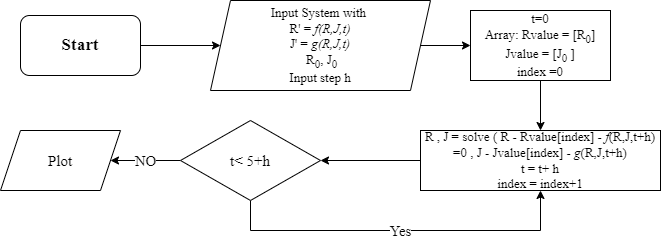
\includegraphics[scale = .6]{Images/Bt4/flowchart.png}
        \caption{Lưu đồ thuật toán}
    \end{figure}
    \newline
    $\indent$ Ta thấy trong việc sử dụng phương pháp Implicit Euler, ta phải thực hiện giải phương trình (ở đây là hệ phương trình). Việc giải một hệ phương trình tổng quát (ở đây $f$ và $g$ có thể không tuyến tính). Để giải hệ này, ta cần có một cặp giá trị dự đoán giá trị nghiệm. Nếu giá trị chúng ta sử dụng để dự đoán càng gần giá trị nghiệm thực tế, việc giải sẽ nhanh và chính xác cao hơn. Ta sẽ sử dụng giá trị dưới đây để dự đoán:
    \begin{equation*}
        \begin{cases}
            R_{i+1} = R_i + hf(R_i,J_i,t_i) \\
            J_{i+1} = J_i + hf(R_i,J_i,t_i)
        \end{cases}
    \end{equation*}
    
    \item \textbf{Hiện thực:} 
    \begin{itemize}
        \item \textbf{Chuẩn bị thư viện}
        \begin{lstlisting}
    import matplotlib.pyplot as plt
    import matplotlib.cm as cm
    import numpy as np
    import sympy as sym
    from scipy.optimize import fsolve
    import warnings
    warnings.filterwarnings('ignore', 'The iteration is not making good progress')
        \end{lstlisting}
        \item \textbf{Nhập đầu vào}
        \begin{lstlisting}
    R = sym.Symbol('\dot{R})
    J = sym.Symbol('\dot{J})
    t = sym.Symbol('t')
    expr1 = input("please input the expresion of \dot{R}: \dot{R} = ")
    Rd = sym.lambdify((R,J,t),expr1,"numpy")
    expr2 = input("please input the expression of \dot{J}: \dot{J} = ")
    Jd = sym.lambdify((R,J,t),expr2,"numpy")
    R0 = float(input("please input R0 = "))
    J0 = float(input("please input J0 = "))
    h = float(input("Please input h = "))
        \end{lstlisting}
        \item \textbf{Phương thức vẽ mặt phẳng pha và Explicit method (để so sánh kết quả với Implicit method)}
        \begin{lstlisting}
    def ExplicitEulerMethod():
        def ExplicitEuler(f, g, t0, R0, J0, h):
            R1 = R0 + f(R0, J0,t0) * h
            J1 = J0 + g(R0,J0,t0) * h
            return [R1, J1]
        time = np.arange(0,5+h,h)
        value = []
        Rarray = []
        Jarray = []
        value.append([R0,J0])
        Rarray.append(value[0][0])
        Jarray.append(value[0][1])
        for i in range(0,len(time)-1):
            value.append(ExplicitEuler(Rd,Jd,time[i], value[i][0],value[i][1],h))
            Rarray.append(value[i+1][0])
            Jarray.append(value[i+1][1])
        Rarray=np.array(Rarray)
        Jarray=np.array(Jarray)
        return [Rarray,Jarray]
      
    def vector_field(dR, dJ):
        plt.figure(figsize = (12, 8))
        r_range = j_range = np.linspace(-20, 20, 9)
        r, j = np.meshgrid(r_range, j_range)
        t = 0
        a = dR(1, 0, t)
        b = dR(0, 1, t)
        c = dJ(1, 0, t)
        d = dJ(0, 1, t)
        h = np.sqrt((a**2 + c**2)*r**2 + 2*(a*b + c*d)*r*j + (b**2 + d**2)*j**2)
        fx = dR(r, j, t)
        fy = dJ(r, j, t)
        for m in range(len(r_range)):
            for n in range(len(j_range)):
                if h[m][n] != 0:
                    fx[m][n] = fx[m][n] / h[m][n]
                    fy[m][n] = fy[m][n] / h[m][n]
        colors = np.linspace(0, 1, 9)
        plt.xlabel('Romeo\'s Love for Juliet ')
        plt.ylabel('Juliet \'s Love for Romeo')
        plt.quiver(r, j, fx, fy, pivot = "mid", color = cm.summer(colors))
        plt.axis("scaled")
        plt.show()
        \end{lstlisting}
        \item \textbf{Implicit method}
        \begin{lstlisting}
    def ImplicitEulerMethod():
        time = np.arange(0,5+h,h)
        Rarray = [R0]
        Jarray = [J0]
        index =0 
        for i in range(0,len(time)-1):
            index=i
            def equations(p):
                R, J = p
                return (R-Rarray[index]-h*Rd(R,J,time[index+1]), J-Jarray[index]-h*Jd(R,J,time[index+1]))
            x,y=fsolve(equations,(Rarray[i]+h*Rd(Rarray[i] ,Jarray[i],time[i]) ,Jarray[i]+h*Jd(Rarray[i],Jarray[i],time[i])))
            Rarray.append(float(x))
            Jarray.append(float(y))
        Rarray=np.array(Rarray)
        Jarray=np.array(Jarray)
        return [Rarray,Jarray]
        \end{lstlisting}
        \item \textbf{Plot}
        \begin{lstlisting}
    temp1=ExplicitEulerMethod()
    temp2=ImplicitEulerMethod()
    time = np.arange(0,5+h,h)
    plt.figure(figsize = (10, 8))
    plt.plot(time, temp1[0], '\dot{R}, label='R with Explicit')
    plt.plot(time, temp1[1], 'b', label='J with Explicit')
    plt.plot(time,temp2[0],'y',label ='R with Implicit')
    plt.plot(time,temp2[1],'g',label = 'J with Implicit')
    plt.xlabel('t')
    plt.ylabel('f(t)')
    plt.legend(loc='lower right')
    plt.grid()
    plt.show()
    vector_field(Rd, Jd)
        \end{lstlisting}
    \end{itemize}
    \item \textbf{Ví dụ:}
    \begin{enumerate}
         \item Ví dụ 1:
        \begin{equation} \label{ex:vd1}
            \begin{cases}
            \dot{R} = -3R +3J - sin(e^{t^2}-cos(t))\\
            \dot{J} = -2R + J \\
            R(0) = -4, J(0) = 2
        \end{cases}
    \end{equation}
$\indent$ Ta thấy hệ trên chỉ đơn giản là hệ không thuần nhất với nguyên hàm (\ref{eq:30}) không tồn tại nguyên hàm sơ cấp. Ta giải xấp xị hệ với lần lượt bước nhảy $h=0.1$ và $h=0.01$. Ta được kết quả sau:
\begin{figure}[htp]
    \centering
    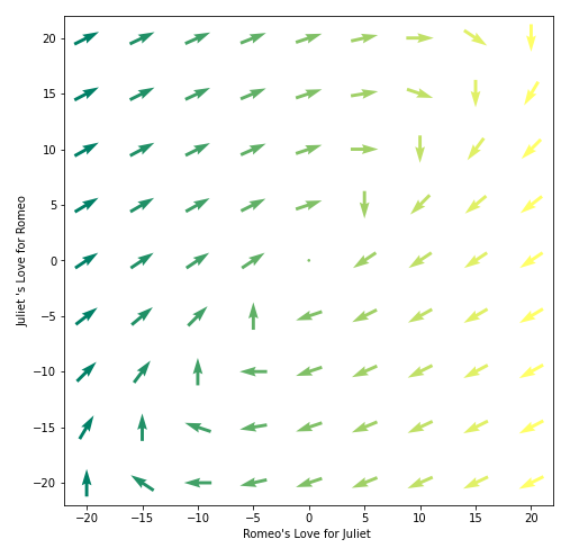
\includegraphics[scale = .8]{Images/Bt4/vd1/field.png}
    \caption{Mặt phẳng pha ví dụ 1}
\end{figure} 
\newpage
\begin{figure}[htp] 
    \begin{tabular}{cc}
        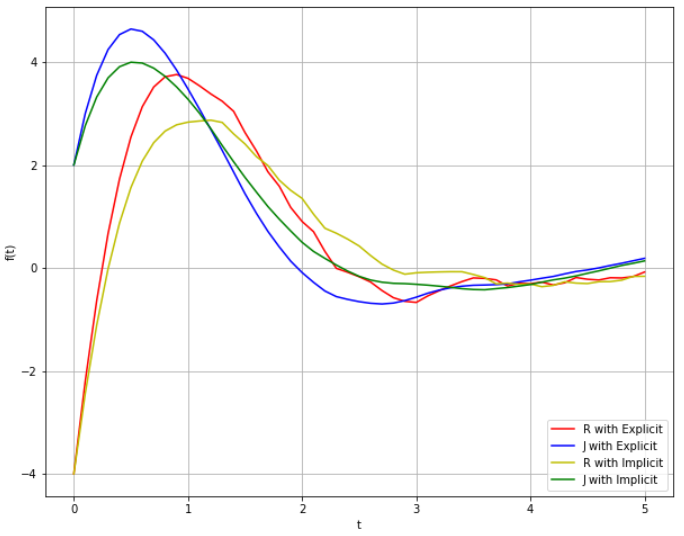
\includegraphics[scale=.58]{Images/Bt4/vd1/h=0,1.png} &
        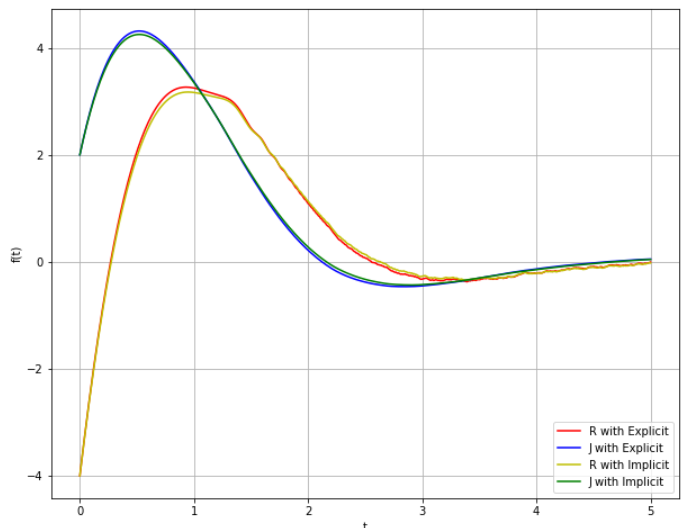
\includegraphics[scale = .58]{Images/Bt4/vd1/h=0.01.png} \\
        h=0.1 & h=0.01
    \end{tabular}
    \caption{Đồ thị theo thời gian ví dụ 1}
    
\end{figure}
$\indent$ Các đường màu đỏ, xanh dương, vàng và xanh lá cây lần lượt là R theo phương pháp Explicit, J theo phương pháp Explicit, R theo phương pháp Implicit và J theo phương pháp Implicit
    \item ví dụ 2:
    \begin{equation} \label{ex:vd2}
        \begin{cases}
            \dot{R}= Rsin(t) + Je^{-t} \\
            \dot{J} = R+Jcos(t) + sin(t^2) \\
            R(0) = 2, J(0) = -3
        \end{cases}
    \end{equation}
    \begin{figure}[htp]
    \centering
    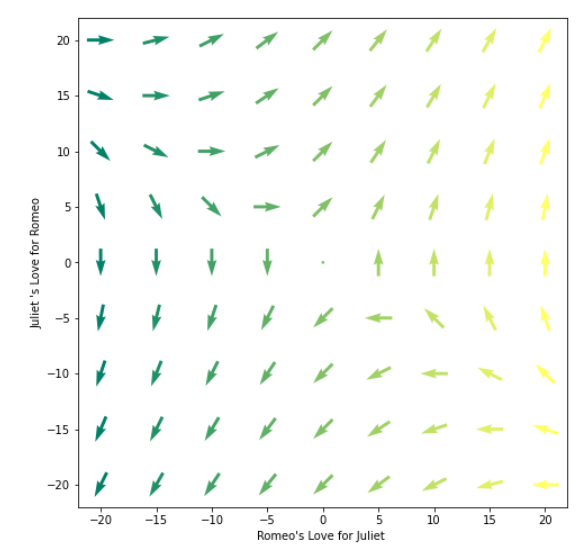
\includegraphics[scale = .8]{Images/Bt4/vd2/field.png}
    \caption{Mặt phẳng pha ví dụ 2}
\end{figure} 
\newpage
\begin{figure}[htp] 
    \begin{tabular}{cc}
        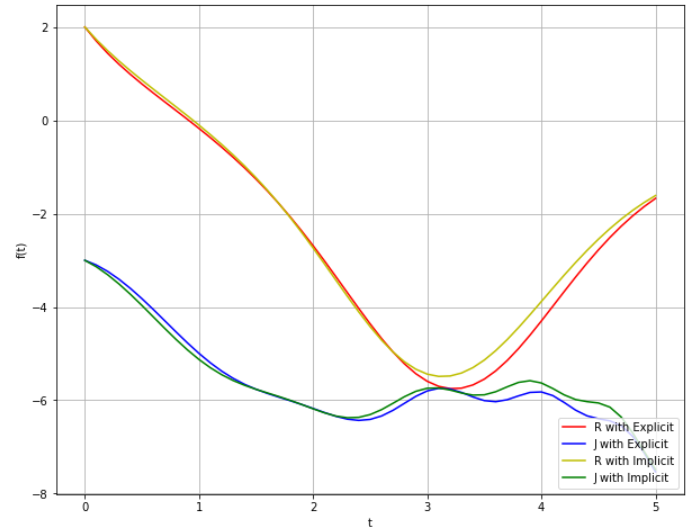
\includegraphics[scale=.58]{Images/Bt4/vd2/h=0,1.png} &
        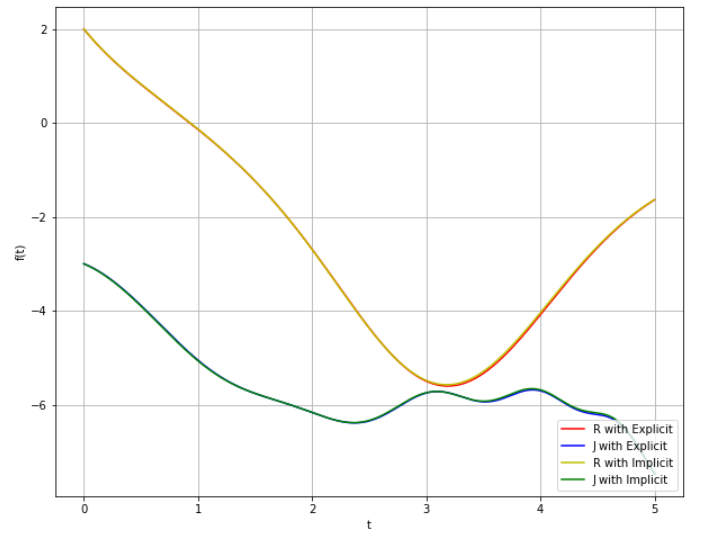
\includegraphics[scale = .58]{Images/Bt4/vd2/h=0.01.png} \\
        h=0.1 & h=0.01
    \end{tabular}
    \caption{Đồ thị theo thời gian ví dụ 2}
\end{figure}

\item ví dụ 3:
    \begin{equation} \label{ex:vd3}
        \begin{cases}
            \dot{R} = sin(R)+cos(J) \\
            \dot{J} = RJtcos(R+J)\\
            R(0) = 1, J(0) = -2
        \end{cases}
    \end{equation}
    \begin{figure}[htp]
    \centering
    \includegraphics[scale = .8]{Images/Bt4/vd3/field.png}
    \caption{Mặt phẳng pha ví dụ 3}
\end{figure} 
\newpage
\begin{figure}[htp] 
    \begin{tabular}{cc}
        \includegraphics[scale=.58]{Images/Bt4/vd3/h=0,2.png} &
        \includegraphics[scale = .58]{Images/Bt4/vd3/h=0.01.png} \\
        h=0.2 & h=0.01
    \end{tabular}
    \caption{Đồ thị theo thời gian ví dụ 3}
\end{figure}

\item ví dụ 4:
    \begin{equation} \label{ex:vd4}
        \begin{cases}
    \dot{R}=Je^{-t}\log(R+40)\\
    \dot{J}=R-t\log(J+40)\\
    R(0)=10,J(0) = -2
        \end{cases}
    \end{equation}
    \begin{figure}[htp]
    \centering
    \includegraphics[scale = .8]{Images/Bt4/vd4/field.png}
    \caption{Mặt phẳng pha ví dụ 2}
\end{figure} 
\newpage
\begin{figure}[htp] 
    \begin{tabular}{cc}
        \includegraphics[scale=.58]{Images/Bt4/vd4/h=0,1.png} &
        \includegraphics[scale = .58]{Images/Bt4/vd4/h=0.01.png} \\
        h=0.1 & h=0.01
    \end{tabular}
    \caption{Đồ thị theo thời gian ví dụ 4}
\end{figure}

 \item ví dụ 5:
    \begin{equation} \label{ex:vd5}
        \begin{cases}
    \dot{R} = \sqrt{(R-t)^2+(J-t)^2}\\
    \dot{J} = t(R-J)\\
    R(0)=-10,J(0) = 10
        \end{cases}
    \end{equation}
    \begin{figure}[htp]
    \centering
    \includegraphics[scale = .8]{Images/Bt4/vd5/field.png}
    \caption{Mặt phẳng pha ví dụ 2}
\end{figure} 
\newpage
\begin{figure}[htp] 
    \begin{tabular}{cc}
        \includegraphics[scale=.58]{Images/Bt4/vd5/h=0,1.png} &
        \includegraphics[scale = .58]{Images/Bt4/vd5/h=0.01.png} \\
        h=0.1 & h=0.01
    \end{tabular}
    \caption{Đồ thị theo thời gian ví dụ 5}
\end{figure}
    \end{enumerate}
    \item \textbf{Nhận xét} \\
    $\indent$ Ta thấy khuyết điểm lớn nhất của phương pháp Implicit Euler chính là việc ta buộc phải giải phương trình (hay ở đây là hệ phương trình). Ta buộc phải bỏ ra tài nguyên về thời gian và không gian để có thể giải tìm nghiệm của hệ và nếu ta cho bước nhảy nhỏ $h$ rât bé, ta sẽ phải giải phương trình liên tục qua mỗi bước. Vậy phương pháp này sẽ phù hợp hơn vái những bài toán sự thay đổi của hàm được thể hiện qua thời gian rất dài. \\
    $\indent$ Ngoài ra, việc dự đoán nghiệm sẽ cần thiết cho việc các thiết bị hỗ trợ có thể giải ra nghiệm một cách chính xác, nếu nghiệm ta dự đoán quá xa nghiệm thực tế, thời gian để giải ra nghiệm thực tế sẽ lâu hơn và độ chính xác cũng thấp hơn.
\end{enumerate} 
\newpage
\subsection{Bài tập 5}
\subsubsection{Nội dung}
$\indent$ Với hệ phương trình vi phân tuyến tính cấp một thuần nhất với hệ sống hằng (\ref{eq:1}), ta có 1000 cặp $R$ và $J$ là các cặp giá trị của một hệ (\ref{eq:1}) và biết tập dữ liệu có các dữ liệu bị nhiễu. Biết giá trị $R_0 = -2 $, $J_0=3$ và các cặp giá trong tập dữ liệu được tạo ra bởi hàm (\ref{eq:1}) với bước nhảy là $0.001$. Ta cần tìm hệ số $a$, $b$, $c$ và $d$ tương ứng của hệ.
\subsubsection{Đặt vấn đề}
$\indent$ Trước khi tìm kiếm mô hình giải quyết bài toán ta trực quan hóa các cặp $R$, $J$ ta được:
\begin{figure}[htp]
    \centering
    \includegraphics{Images/Bt5/noisedata.png}
    \caption{R và J theo thời gian}
\end{figure}
$\indent$ Ta thấy, các dữ liệu nhiễu chính là dữ liệu đúng ứng với hệ cần tìm cộng thêm một thành phần sai số.
\begin{equation} \label{eq:5.2_1}
    \begin{cases}
        R_i = \hat{R_i} + \epsilon_{Ri} \\
        J_i = \hat{J_i} + \epsilon_{Ji}
    \end{cases}
\end{equation}
Với $\hat{R_i}$, $\hat{R_j}$ là các giá trị ta ướng lượng cho R và J khi xác định các hệ số $a$, $b$, $c$, $d$. $R_i$ và $J_i$ là các cặp R và J tương ứng. $\epsilon$ là các thành phần sai số. Để có thể tìm các hệ số $a$, $b$, $c$ và $d$, ta mong muốn với các hệ số đó, nghiệm của hệ sẽ làm cho tổng thành phần sai số là nhỏ nhất hay trung bình bình phương thành phần sai số là nhỏ nhất. Nghĩa là ta mong muốn rằng: \\
\begin{equation} \label{loss_function}
    \left[f(a,b,c,d) = \frac{\displaystyle \sum_{i=1}^{1000}\epsilon_{Ri} +\displaystyle \sum_{i=1}^{1000}\epsilon_{Ji} }{1000} \right]_{min}
\end{equation}
$\indent$ Ta cần xây dựng mô hình đề tìm giá trị nhỏ nhất của $f(a,b,c,d)$.
\subsubsection{Mô hình Gradient Descent}
$\indent$ Với bài toán đặt ra ta sẽ khó tìm được giá trị nhỏ nhất của hàm số trên toàn tập xác định, ta sẽ cố gắng tìm một giá trị cực tiểu trong một lân cận nào đó và mong rằng đó chính là giá trị chúng ta đang tìm kiếm.\\
$\indent$ Với lý thuyết về hàm đa biến ta có, vector gradient của hàm số $\triangledown f = \left(\frac{\partial f}{\partial x_1} , \dots, \frac{\partial f}{\partial x_n} \right)^T$ là một trường vector thể hiện chiều hướng tăng lớn nhất của $f$. Vậy nếu ta đi ngược chiều của $\triangledown f$, ta sẽ đang đi về hướng có độ giảm nhanh nhất và ta mong rằng khi càng tiến theo hướng đó, ta sẽ càng đi lại gần giá trị cực tiểu địa phương và đó sẽ là giá trị ta cần tìm.\\
$\indent$ Ta thấy hàm $f(a,b,c,d)$ không có công thức tườnng minh để tính đạo hàm, vì thế ta tính đạo hàm riêng theo công thức:
\begin{equation}
    \frac{\partial f}{\partial a} = \displaystyle  \lim_{h \to 0} \frac{f(a+h,b,c,d)-f(a,b,c,d)}{h}
\end{equation}
$\indent$ Ta có lưu đồ sau: 
\begin{figure}[htp]
    \centering
    \includegraphics[scale = .6]{Images/Bt5/flowchart.png}
    \caption{Lưu đồ mô hình Gradient Descent}
\end{figure}
\newline
$\indent$ Trong lưu đồ trên ta có $\delta$ là điều kiện dựng, $\eta$ lạ một hệ số gọi là learning rate. Ở bài tập này, ta chọn $\delta = 0.05$ và $\eta =  0.001$. Dưa vào biểu đồ của $R$ và $J$ theo thời gian ta thấy R và J giảm dần trong thời gian từ 0 đến 1, vì thế ta chọn các giá trị dự đoán $a=2$, $b=1$, $c=4$, $d=3$.
\subsubsection{Hiện thực mô hình}
\begin{enumerate}
    \item \textbf{Chuẩn bị thư viện và đọc dữ liệu}
    \begin{lstlisting}
    import matplotlib.pyplot as plt
    import matplotlib.cm as cm
    import numpy as np
    import pandas as pd
    from sklearn.metrics import mean_squared_error
    df = pd.read_excel('exact.xlsx')
    \end{lstlisting}
    \item \textbf{Tính giá trị cặp R, J tương ứng với a, b, c, d (dùng các công thức ở bài tập 1)}
    \begin{lstlisting}
    def functionValue(a,b,c,d,R0,J0):
      delta = (a-d)**2+4*b*c
      R = []
      J = []
      t = np.arange(0,1,0.001)
      if delta > 0:
        for i in range(len(t)):
          R.append(-1*(2*b*J0+R0*(a-d-np.sqrt((a-d)**2+4*b*c)))/ (2*np.sqrt((a-d)**2+4*b*c))* np.e**(t[i]*(a+d-np.sqrt((a-d)**2+4*b*c))/2) +(2*b*J0+R0*(a-d+np.sqrt((a-d)**2+4*b*c)))/ (2*np.sqrt((a-d)**2+4*b*c)) *np.e**(t[i]*(a+d+np.sqrt((a-d)**2+4*b*c))/2))
          J.append(((np.sqrt((a-d)**2+4*b*c)+a-d)* (2*b*J0+R0*(a-d-np.sqrt((a-d)**2+4*b*c))))/ (4*b*np.sqrt((a-d)**2+4*b*c))* np.e**(t[i]*(a+d-np.sqrt((a-d)**2+4*b*c))/2) +((np.sqrt((a-d)**2+4*b*c)-a+d)*(2*b*J0+R0* (a-d+np.sqrt((a-d)**2+4*b*c))))/(4*b*np.sqrt((a-d)**2+4*b*c))* np.e**(t[i]*(a+d+np.sqrt((a-d)**2+4*b*c))/2))
      elif delta ==0:
        C1 = b*J0 + R0*(a - d)/2
        C2 = J0*(d-a) - R0*(d-a)**2/(4*b)
        for i in range(len(t)):
          R.append((C1 * t + R0)*np.e**(t[i] * (a+d)/2))
          J.append((C2 * t + J0)*np.e**(t[i] * (a+d)/2))
      else:
        C1 = (2*b*J0 - (d-a)*R0) / (np.sqrt(-1*delta))
        C2 = ((d-a)*J0 + 2*c*R0) / (np.sqrt(-1*delta))
        for i in range(len(t)):
          R.append((np.e**(t[i]*(a+d)/2))*(R0*np.cos(t[i] * np.sqrt(-1*delta)/2) + C1*np.sin(t[i] * np.sqrt(-1*delta)/2)))
          J.append((np.e**(t[i]*(a+d)/2) )*(J0*np.cos(t[i] * np.sqrt(-1*delta)/2) + C2*np.sin(t[i] * np.sqrt(-1*delta)/2)))
      R=np.array(R)
      J=np.array(J)
      return R,J 
    \end{lstlisting}
    \item \textbf{Tổng trung bình bình phương sai số}
    \begin{lstlisting}
    def totalError(approxR,approxJ,realR,realJ):
      return mean_squared_error(realR, approxR)+mean_squared_error(realJ, approxJ)
    \end{lstlisting}
    \item \textbf{Tính toán đạo hàm}
    \begin{lstlisting}
    def gradiant(a,b,c,d,R0,J0,h,approxR,approxJ,realR,realJ):
      initialState = totalError(approxR,approxJ,realR,realJ)
      temp1, temp2 = functionValue(a+h,b,c,d,R0,J0)
      dA = (totalError(approxR,approxJ,temp1,temp2)-initialState)/h
      temp1, temp2 = functionValue(a,b+h,c,d,R0,J0)
      dB =  (totalError(approxR,approxJ,temp1,temp2)-initialState)/h
      temp1, temp2 = functionValue(a,b,c+h,d,R0,J0)
      dC =  (totalError(approxR,approxJ,temp1,temp2)-initialState)/h
      temp1, temp2 = functionValue(a,b,c,d+h,R0,J0)
      dD =  (totalError(approxR,approxJ,temp1,temp2)-initialState)/h
      return [dA,dB,dC,dD]
    \end{lstlisting}
    \item \textbf{Gradient Descent}
    \begin{lstlisting}
    approxR = df['\dot{R}]
    approxJ = df['\dot{J}]
    a0 = 2.0
    b0 = 1.0
    c0 = 4.0
    d0 = 3.0
    R0 = -2.0
    J0 = 3.0
    h = 1e-6
    learningRate = 0.001
    while True:
      realR, realJ = functionValue(a0,b0,c0,d0,R0,J0)
      grad = gradiant(a0,b0,c0,d0,R0,J0,h,approxR,approxJ,realR,realJ)
      print(grad) #theo doi gia tri grad
      if (np.abs(grad[0]) < 0.05 and np.abs(grad[1]) < 0.05 and np.abs(grad[2]) < 0.05 and np.abs(grad[3]) < 0.05):
        break
      a0 -= learningRate*grad[0]
      b0 -=learningRate*grad[1]
      c0 -= learningRate*grad[2]
      d0 -= learningRate*grad[3]
    print(a0,b0,c0,d0)
    \end{lstlisting}
\end{enumerate}
\subsubsection{Kết quả}
$\indent$ Tổng thời gian thực thi: 49 phút\\
$\indent$ \textbf{Kết quả thu được: }
\begin{equation*}
    \begin{matrix}
        a & = & 2.423599035087152\\
        b & = & 3.41511738723843\\
        c & = & 5.157800189081293\\
        d & = & -1.855808628080327
    \end{matrix}
\end{equation*}
$\indent$ Đồ thị R và J theo t:
\begin{figure}[htp]
    \centering
    \includegraphics{Images/Bt5/predict.png}
    \caption{Đồ thị R và J theo t}
\end{figure}
\newline
$\indent$ \textbf{Kiểm định kết quả:} \\
$\indent$ Tổng trung bình bình phương sai số: $1.9198012235942574$\\
$\indent$ Tổng trung bình bình phương sai số đối với R: $0.9827149833373434$\\
$\indent$ Tổng trung bình bình phương sai số đối với J: $0.9370862402569139$ \\
$\indent$ Giá trị gradient tại kết quả: 
\begin{equation*}
    \triangledown f = \begin{pmatrix}
        0.01790766357423479 \\ 
        -0.02573516821868793\\
        -0.03624214528485936 \\ 
        0.049996032869259466
    \end{pmatrix}
\end{equation*}
$\indent$ Kiểm tra mối quan hệ tuyến tính của R và và J:
\begin{figure}[htp]
    \centering
    \includegraphics{Images/Bt5/linear.png}
    \caption{Mối quan hệ của R và J}
\end{figure}
\newline
$\indent$ Kiểm tra độ khớp với dữ liệu: \\
Đối với R:
\begin{figure}[htp]
    \centering
    \includegraphics{Images/Bt5/Rfitted.png}
    \caption{Độ khớp của R}

\end{figure}
\newpage

Đối với J:
\begin{figure} [htp]
    \centering
    \includegraphics{Images/Bt5/Jfitted.png}
    \caption{Độ khớp của J}

\end{figure}
\newline
$\indent$ \textbf{Kết luận:} \\
$\indent$ Với giá trị a, b, c, d ta thu được, ta thấy dữ liệu với độ khớp cao, ta có thể giảm learning rate và giảm điều kiện dừng để thu được kết quả chính xác hơn. \\
$\indent$ Các giá trị a, b, c, d ta tìm được là một trong những giá trị a, b, c, d thỏa tính chất của tập dữ liệu.
\newpage
\begin{thebibliography}{80}
\bibitem{bib1}
Vladimir I Arnold. \emph{Ordinary Differential Equations.}   Springer Science \& Business Media, 1992.
\bibitem{bib2}
Tamirat Temesgen Dufera. Deep neural network for system of ordinary differential equa-
tions: Vectorized algorithm and simulation. \emph{Machine Learning with Applications}, 5:100058, 2021.
\bibitem{bib3}
Morris W Hirsch and Stephen Smale. \emph{Differential Equations, Dynamical Systems, and Linear Algebra.} Academic Press, 1974.
\bibitem{bib4}
David G Luenberger. \emph{Introduction to Dynamic Systems: Theory, Models, and Applications}, volume 1. Wiley New York, 1979.
\bibitem{bib5}
Duc Q Nguyen, Nghia Q Vo, Thinh T Nguyen, Khuong Nguyen-An, Quang H Nguyen, Dang N Tran, and Tho T Quan. Becaked: An explainable artificial intelligence model for covid-19 forecasting. \emph{Scientific Reports}, 12(1):1–26, 2022.
\bibitem{bib6}
Steven H Strogatz. Love affairs and differential equations. \emph{Mathematics Magazine}, 61(1):35–35, 1988.
\bibitem{bib7}
References of Exercise (\ref{ex:3}) in 
\href{www.mat.univie.ac.at/~gerald/ftp/book-ode/ode.pdf}{\nolinkurl{here}}
,
\href{https://math.stackexchange.com/questions/347599/questions-about-the-picard-lindel%C3%B6f-theorem-for-an-ode}{\nolinkurl{here}}
or
\href{https://www.sciencedirect.com/topics/mathematics/nonhomogeneous-linear-system}{\nolinkurl{here}}
\end{thebibliography}
\end{document}

